\documentclass[twoside]{book}

% Packages required by doxygen
\usepackage{fixltx2e}
\usepackage{calc}
\usepackage{doxygen}
\usepackage[export]{adjustbox} % also loads graphicx
\usepackage{graphicx}
\usepackage[utf8]{inputenc}
\usepackage{makeidx}
\usepackage{multicol}
\usepackage{multirow}
\PassOptionsToPackage{warn}{textcomp}
\usepackage{textcomp}
\usepackage[nointegrals]{wasysym}
\usepackage[table]{xcolor}

% Font selection
\usepackage[T1]{fontenc}
\usepackage[scaled=.90]{helvet}
\usepackage{courier}
\usepackage{amssymb}
\usepackage{sectsty}
\renewcommand{\familydefault}{\sfdefault}
\allsectionsfont{%
  \fontseries{bc}\selectfont%
  \color{darkgray}%
}
\renewcommand{\DoxyLabelFont}{%
  \fontseries{bc}\selectfont%
  \color{darkgray}%
}
\newcommand{\+}{\discretionary{\mbox{\scriptsize$\hookleftarrow$}}{}{}}

% Page & text layout
\usepackage{geometry}
\geometry{%
  a4paper,%
  top=2.5cm,%
  bottom=2.5cm,%
  left=2.5cm,%
  right=2.5cm%
}
\tolerance=750
\hfuzz=15pt
\hbadness=750
\setlength{\emergencystretch}{15pt}
\setlength{\parindent}{0cm}
\setlength{\parskip}{0.2cm}
\makeatletter
\renewcommand{\paragraph}{%
  \@startsection{paragraph}{4}{0ex}{-1.0ex}{1.0ex}{%
    \normalfont\normalsize\bfseries\SS@parafont%
  }%
}
\renewcommand{\subparagraph}{%
  \@startsection{subparagraph}{5}{0ex}{-1.0ex}{1.0ex}{%
    \normalfont\normalsize\bfseries\SS@subparafont%
  }%
}
\makeatother

% Headers & footers
\usepackage{fancyhdr}
\pagestyle{fancyplain}
\fancyhead[LE]{\fancyplain{}{\bfseries\thepage}}
\fancyhead[CE]{\fancyplain{}{}}
\fancyhead[RE]{\fancyplain{}{\bfseries\leftmark}}
\fancyhead[LO]{\fancyplain{}{\bfseries\rightmark}}
\fancyhead[CO]{\fancyplain{}{}}
\fancyhead[RO]{\fancyplain{}{\bfseries\thepage}}
\fancyfoot[LE]{\fancyplain{}{}}
\fancyfoot[CE]{\fancyplain{}{}}
\fancyfoot[RE]{\fancyplain{}{\bfseries\scriptsize Generated on Mon Apr 11 2016 23\+:11\+:10 for Capstone by Doxygen }}
\fancyfoot[LO]{\fancyplain{}{\bfseries\scriptsize Generated on Mon Apr 11 2016 23\+:11\+:10 for Capstone by Doxygen }}
\fancyfoot[CO]{\fancyplain{}{}}
\fancyfoot[RO]{\fancyplain{}{}}
\renewcommand{\footrulewidth}{0.4pt}
\renewcommand{\chaptermark}[1]{%
  \markboth{#1}{}%
}
\renewcommand{\sectionmark}[1]{%
  \markright{\thesection\ #1}%
}

% Indices & bibliography
\usepackage{natbib}
\usepackage[titles]{tocloft}
\setcounter{tocdepth}{3}
\setcounter{secnumdepth}{5}
\makeindex

% Hyperlinks (required, but should be loaded last)
\usepackage{ifpdf}
\ifpdf
  \usepackage[pdftex,pagebackref=true]{hyperref}
\else
  \usepackage[ps2pdf,pagebackref=true]{hyperref}
\fi
\hypersetup{%
  colorlinks=true,%
  linkcolor=blue,%
  citecolor=blue,%
  unicode%
}

% Custom commands
\newcommand{\clearemptydoublepage}{%
  \newpage{\pagestyle{empty}\cleardoublepage}%
}


%===== C O N T E N T S =====

\begin{document}

% Titlepage & ToC
\hypersetup{pageanchor=false,
             bookmarks=true,
             bookmarksnumbered=true,
             pdfencoding=unicode
            }
\pagenumbering{roman}
\begin{titlepage}
\vspace*{7cm}
\begin{center}%
{\Large Capstone }\\
\vspace*{1cm}
{\large Generated by Doxygen 1.8.9.1}\\
\vspace*{0.5cm}
{\small Mon Apr 11 2016 23:11:10}\\
\end{center}
\end{titlepage}
\clearemptydoublepage
\tableofcontents
\clearemptydoublepage
\pagenumbering{arabic}
\hypersetup{pageanchor=true}

%--- Begin generated contents ---
\chapter{Capstone}
\label{index}\hypertarget{index}{}\hypertarget{index_intro_sec}{}\section{Introduction}\label{index_intro_sec}
\begin{DoxyVerb}     ....
\end{DoxyVerb}
\hypertarget{index_install_sec}{}\section{Installation}\label{index_install_sec}
\begin{DoxyVerb}     ....\end{DoxyVerb}
 
\chapter{wm}
\label{md_README}
\hypertarget{md_README}{}
\input{md_README}
\chapter{Class Index}
\section{Class List}
Here are the classes, structs, unions and interfaces with brief descriptions\+:\begin{DoxyCompactList}
\item\contentsline{section}{\hyperlink{structNode}{Node} }{\pageref{structNode}}{}
\item\contentsline{section}{\hyperlink{structWorkspace}{Workspace} }{\pageref{structWorkspace}}{}
\end{DoxyCompactList}

\chapter{File Index}
\section{File List}
Here is a list of all files with brief descriptions\+:\begin{DoxyCompactList}
\item\contentsline{section}{\hyperlink{config_8h}{config.\+h} }{\pageref{config_8h}}{}
\item\contentsline{section}{\hyperlink{keys_8h}{keys.\+h} }{\pageref{keys_8h}}{}
\item\contentsline{section}{\hyperlink{linkedlist_8c}{linkedlist.\+c} }{\pageref{linkedlist_8c}}{}
\item\contentsline{section}{\hyperlink{linkedlist_8h}{linkedlist.\+h} }{\pageref{linkedlist_8h}}{}
\item\contentsline{section}{\hyperlink{mytilewm_8c}{mytilewm.\+c} }{\pageref{mytilewm_8c}}{}
\item\contentsline{section}{\hyperlink{utils_8h}{utils.\+h} }{\pageref{utils_8h}}{}
\end{DoxyCompactList}

\chapter{Class Documentation}
\hypertarget{structNode}{}\section{Node Struct Reference}
\label{structNode}\index{Node@{Node}}


{\ttfamily \#include $<$linkedlist.\+h$>$}



Collaboration diagram for Node\+:\nopagebreak
\begin{figure}[H]
\begin{center}
\leavevmode
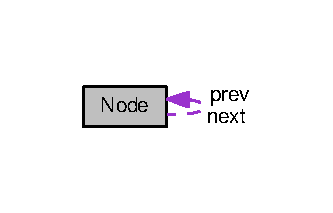
\includegraphics[width=160pt]{structNode__coll__graph}
\end{center}
\end{figure}
\subsection*{Public Attributes}
\begin{DoxyCompactItemize}
\item 
Window \hyperlink{structNode_a9b48ab73d4bb7a253057af4aaa165a1d}{win\+I\+D}
\item 
Window \hyperlink{structNode_a58ff43cedbc9c788aa1298715042768d}{decoration}
\item 
int \hyperlink{structNode_ac759c6f57f027e265a5e369a69114479}{floating}
\item 
int \hyperlink{structNode_a9f51700be8fa8a1e0c032f0f18f9f744}{mapped}
\item 
int \hyperlink{structNode_ab914f0acd82df7f22818d31337442792}{transient}
\item 
\hyperlink{structNode}{Node} $\ast$ \hyperlink{structNode_a632ea91c6a13082308f7692649a68880}{prev}
\item 
\hyperlink{structNode}{Node} $\ast$ \hyperlink{structNode_a2559a716f69ccaa76d648d9f1b83065e}{next}
\end{DoxyCompactItemize}


\subsection{Detailed Description}
Functions for manipulating a doubly, circular linked list holding X\+Lib Window I\+Ds. A \hyperlink{structNode}{Node} in a circular, doubly linked list. Represents an X\+Lib Window, and holds some extra information about the window\textquotesingle{}s current state. 

\subsection{Member Data Documentation}
\hypertarget{structNode_a58ff43cedbc9c788aa1298715042768d}{}\index{Node@{Node}!decoration@{decoration}}
\index{decoration@{decoration}!Node@{Node}}
\subsubsection[{decoration}]{\setlength{\rightskip}{0pt plus 5cm}Window Node\+::decoration}\label{structNode_a58ff43cedbc9c788aa1298715042768d}
\hypertarget{structNode_ac759c6f57f027e265a5e369a69114479}{}\index{Node@{Node}!floating@{floating}}
\index{floating@{floating}!Node@{Node}}
\subsubsection[{floating}]{\setlength{\rightskip}{0pt plus 5cm}int Node\+::floating}\label{structNode_ac759c6f57f027e265a5e369a69114479}
\hypertarget{structNode_a9f51700be8fa8a1e0c032f0f18f9f744}{}\index{Node@{Node}!mapped@{mapped}}
\index{mapped@{mapped}!Node@{Node}}
\subsubsection[{mapped}]{\setlength{\rightskip}{0pt plus 5cm}int Node\+::mapped}\label{structNode_a9f51700be8fa8a1e0c032f0f18f9f744}
\hypertarget{structNode_a2559a716f69ccaa76d648d9f1b83065e}{}\index{Node@{Node}!next@{next}}
\index{next@{next}!Node@{Node}}
\subsubsection[{next}]{\setlength{\rightskip}{0pt plus 5cm}{\bf Node}$\ast$ Node\+::next}\label{structNode_a2559a716f69ccaa76d648d9f1b83065e}
\hypertarget{structNode_a632ea91c6a13082308f7692649a68880}{}\index{Node@{Node}!prev@{prev}}
\index{prev@{prev}!Node@{Node}}
\subsubsection[{prev}]{\setlength{\rightskip}{0pt plus 5cm}{\bf Node}$\ast$ Node\+::prev}\label{structNode_a632ea91c6a13082308f7692649a68880}
\hypertarget{structNode_ab914f0acd82df7f22818d31337442792}{}\index{Node@{Node}!transient@{transient}}
\index{transient@{transient}!Node@{Node}}
\subsubsection[{transient}]{\setlength{\rightskip}{0pt plus 5cm}int Node\+::transient}\label{structNode_ab914f0acd82df7f22818d31337442792}
\hypertarget{structNode_a9b48ab73d4bb7a253057af4aaa165a1d}{}\index{Node@{Node}!win\+I\+D@{win\+I\+D}}
\index{win\+I\+D@{win\+I\+D}!Node@{Node}}
\subsubsection[{win\+I\+D}]{\setlength{\rightskip}{0pt plus 5cm}Window Node\+::win\+I\+D}\label{structNode_a9b48ab73d4bb7a253057af4aaa165a1d}


The documentation for this struct was generated from the following file\+:\begin{DoxyCompactItemize}
\item 
\hyperlink{linkedlist_8h}{linkedlist.\+h}\end{DoxyCompactItemize}

\hypertarget{structWorkspace}{}\section{Workspace Struct Reference}
\label{structWorkspace}\index{Workspace@{Workspace}}


The documentation for this struct was generated from the following file\+:\begin{DoxyCompactItemize}
\item 
\hyperlink{mytilewm_8c}{mytilewm.\+c}\end{DoxyCompactItemize}

\chapter{File Documentation}
\hypertarget{config_8h}{}\section{config.\+h File Reference}
\label{config_8h}\index{config.\+h@{config.\+h}}
This graph shows which files directly or indirectly include this file\+:\nopagebreak
\begin{figure}[H]
\begin{center}
\leavevmode
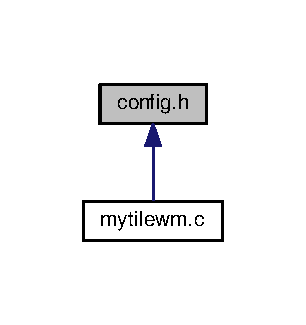
\includegraphics[width=147pt]{config_8h__dep__incl}
\end{center}
\end{figure}
\subsection*{Macros}
\begin{DoxyCompactItemize}
\item 
\#define \hyperlink{config_8h_a6d0652ae6ea6a5c4fef68baf139fd085}{B\+O\+R\+D\+E\+R}~3
\item 
\#define \hyperlink{config_8h_aaf1a851b2560399155b3d31b94b7b5df}{G\+A\+P\+S}~1
\item 
\#define \hyperlink{config_8h_a4c57f55c1caa2238d4f88c656e39e484}{G\+A\+P\+S\+I\+Z\+E}~10
\item 
\#define \hyperlink{config_8h_abe6b939dec8d3b43ba83c53d2d3a3cf6}{G\+A\+P\+S\+\_\+\+I\+N\+C}~3
\item 
\#define \hyperlink{config_8h_a558c51e4f5ec11d7d66ccc3fa5bb64e9}{P\+A\+N\+E\+L}~0
\item 
\#define \hyperlink{config_8h_ad94f97286bd6f40f75df2736a63ac899}{P\+A\+N\+E\+L\+\_\+\+H\+E\+I\+G\+H\+T}~16
\item 
\#define \hyperlink{config_8h_afc370cb702541c6850620907857be1a7}{R\+E\+S\+I\+Z\+E\+\_\+\+I\+N\+C}~10
\item 
\#define \hyperlink{config_8h_a7ed7c989849bb05c71d617e73cd05311}{N\+U\+M\+\_\+\+W\+O\+R\+K\+S\+P\+A\+C\+E\+S}~3
\item 
\#define \hyperlink{config_8h_a70ec4032d37207df82e878c74a919204}{F\+O\+C\+U\+S\+E\+D}~\char`\"{}\#989898\char`\"{}
\item 
\#define \hyperlink{config_8h_aaf31d3d5c2218a7b81427f0034238247}{U\+N\+F\+O\+C\+U\+S\+E\+D}~\char`\"{}\#3c3b37\char`\"{}
\item 
\#define \hyperlink{config_8h_adce122f566c88a1eceeb79a635afa964}{G\+R\+E\+Y}~\char`\"{}\#3c3b37\char`\"{}
\item 
\#define \hyperlink{config_8h_a7b3b25cba33b07c303f3060fe41887f6}{B\+L\+A\+C\+K}~\char`\"{}\#000000\char`\"{}
\item 
\#define \hyperlink{config_8h_ac2544c8b4fe3113b0d6bb62530692c21}{R\+E\+T}~65293
\item 
\#define \hyperlink{config_8h_ad58a1fbfc85c7e4790fc55e654f50221}{T\+A\+B}~65289
\item 
\#define \hyperlink{config_8h_a3d725a80a1060b97c063eac27c4feb60}{S\+P\+C}~32
\item 
\#define \hyperlink{config_8h_aaa0cb465a0693c23b45d0cd8f25224e7}{a\+\_\+\+K\+E\+Y}~97
\item 
\#define \hyperlink{config_8h_aa1fc6e4ef56672d104022864dc8a29ff}{d\+\_\+\+K\+E\+Y}~100
\item 
\#define \hyperlink{config_8h_a221d0119b8b1e01435a1704cdf144b5d}{e\+\_\+\+K\+E\+Y}~101
\item 
\#define \hyperlink{config_8h_a57fc86f319df4caf6a05b899a73df816}{f\+\_\+\+K\+E\+Y}~102
\item 
\#define \hyperlink{config_8h_a5a037cbb50169bd806b8216f6539a14a}{m\+\_\+\+K\+E\+Y}~109
\item 
\#define \hyperlink{config_8h_a86009c371275240cb817091f992dda7f}{q\+\_\+\+K\+E\+Y}~113
\item 
\#define \hyperlink{config_8h_a75ac3acba95812a4be896446cd3051b4}{R\+\_\+\+K\+E\+Y}~82
\item 
\#define \hyperlink{config_8h_a80fb826a684cf3f0d306b22aa100ddac}{R\+I\+G\+H\+T}~65363
\item 
\#define \hyperlink{config_8h_a437ef08681e7210d6678427030446a54}{L\+E\+F\+T}~65361
\item 
\#define \hyperlink{config_8h_a1965eaca47dbf3f87acdafc2208f04eb}{U\+P}~65362
\item 
\#define \hyperlink{config_8h_a4193cd1c8c2e6ebd0e056fa2364a663f}{D\+O\+W\+N}~65364
\item 
\#define \hyperlink{config_8h_a5381a445a1e4bdc36460151d82eed95a}{M\+I\+N\+U\+S}~45
\item 
\#define \hyperlink{config_8h_a214c717b2e51e1993a749ac99df7de58}{E\+Q\+U\+A\+L}~61
\item 
\#define \hyperlink{config_8h_ae27a03218878a9af9d7d946e186f8598}{G\+R\+E\+A\+T\+E\+R}~62
\item 
\#define \hyperlink{config_8h_a16bcdd65ecdd3313af9e393538fa7fa8}{L\+E\+S\+S}~60
\item 
\#define \hyperlink{config_8h_a2b2504f8501ad0cf37e7026794b83741}{B\+R\+A\+C\+K\+E\+T\+\_\+\+L\+E\+F\+T}~91
\item 
\#define \hyperlink{config_8h_a6656d6e13a621b7a6c0a016462683ba8}{B\+R\+A\+C\+K\+E\+T\+\_\+\+R\+I\+G\+H\+T}~93
\item 
\#define \hyperlink{config_8h_a9d8a33b1a8b82b9913a0ba70438d45be}{A\+L\+T}~Mod1\+Mask
\item 
\#define \hyperlink{config_8h_ac179eef68bcc694aa0ef8dd1eb09950b}{S\+H\+I\+F\+T}~Shift\+Mask
\item 
\#define \hyperlink{config_8h_af5bcf329d3c9613928c46e186752d618}{C\+T\+R\+L}~Control\+Mask
\item 
\#define \hyperlink{config_8h_a34ec0bf4b9f4cbde166aa283c8f5b1f2}{S\+U\+P\+E\+R}~Mod4\+Mask
\item 
\#define \hyperlink{config_8h_ab19a74cdecfe8fdf5ec475457079fad0}{T\+E\+R\+M}~\char`\"{}urxvt\&\char`\"{}
\item 
\#define \hyperlink{config_8h_a753face9617b86b15ac0ffd9a2a32c2f}{B\+R\+O\+W\+S\+E\+R}~\char`\"{}firefox\&\char`\"{}
\item 
\#define \hyperlink{config_8h_a17006df43dac0536598494c8e69c0727}{F\+I\+L\+E\+M\+A\+N}~\char`\"{}thunar\&\char`\"{}
\item 
\#define \hyperlink{config_8h_a397d2dfb6f85ff80d24aed448cec57fc}{L\+A\+U\+N\+C\+H\+E\+R}~\char`\"{}rofi -\/show run\char`\"{}
\end{DoxyCompactItemize}


\subsection{Macro Definition Documentation}
\hypertarget{config_8h_aaa0cb465a0693c23b45d0cd8f25224e7}{}\index{config.\+h@{config.\+h}!a\+\_\+\+K\+E\+Y@{a\+\_\+\+K\+E\+Y}}
\index{a\+\_\+\+K\+E\+Y@{a\+\_\+\+K\+E\+Y}!config.\+h@{config.\+h}}
\subsubsection[{a\+\_\+\+K\+E\+Y}]{\setlength{\rightskip}{0pt plus 5cm}\#define a\+\_\+\+K\+E\+Y~97}\label{config_8h_aaa0cb465a0693c23b45d0cd8f25224e7}
\hypertarget{config_8h_a9d8a33b1a8b82b9913a0ba70438d45be}{}\index{config.\+h@{config.\+h}!A\+L\+T@{A\+L\+T}}
\index{A\+L\+T@{A\+L\+T}!config.\+h@{config.\+h}}
\subsubsection[{A\+L\+T}]{\setlength{\rightskip}{0pt plus 5cm}\#define A\+L\+T~Mod1\+Mask}\label{config_8h_a9d8a33b1a8b82b9913a0ba70438d45be}
\hypertarget{config_8h_a7b3b25cba33b07c303f3060fe41887f6}{}\index{config.\+h@{config.\+h}!B\+L\+A\+C\+K@{B\+L\+A\+C\+K}}
\index{B\+L\+A\+C\+K@{B\+L\+A\+C\+K}!config.\+h@{config.\+h}}
\subsubsection[{B\+L\+A\+C\+K}]{\setlength{\rightskip}{0pt plus 5cm}\#define B\+L\+A\+C\+K~\char`\"{}\#000000\char`\"{}}\label{config_8h_a7b3b25cba33b07c303f3060fe41887f6}
\hypertarget{config_8h_a6d0652ae6ea6a5c4fef68baf139fd085}{}\index{config.\+h@{config.\+h}!B\+O\+R\+D\+E\+R@{B\+O\+R\+D\+E\+R}}
\index{B\+O\+R\+D\+E\+R@{B\+O\+R\+D\+E\+R}!config.\+h@{config.\+h}}
\subsubsection[{B\+O\+R\+D\+E\+R}]{\setlength{\rightskip}{0pt plus 5cm}\#define B\+O\+R\+D\+E\+R~3}\label{config_8h_a6d0652ae6ea6a5c4fef68baf139fd085}
\hypertarget{config_8h_a2b2504f8501ad0cf37e7026794b83741}{}\index{config.\+h@{config.\+h}!B\+R\+A\+C\+K\+E\+T\+\_\+\+L\+E\+F\+T@{B\+R\+A\+C\+K\+E\+T\+\_\+\+L\+E\+F\+T}}
\index{B\+R\+A\+C\+K\+E\+T\+\_\+\+L\+E\+F\+T@{B\+R\+A\+C\+K\+E\+T\+\_\+\+L\+E\+F\+T}!config.\+h@{config.\+h}}
\subsubsection[{B\+R\+A\+C\+K\+E\+T\+\_\+\+L\+E\+F\+T}]{\setlength{\rightskip}{0pt plus 5cm}\#define B\+R\+A\+C\+K\+E\+T\+\_\+\+L\+E\+F\+T~91}\label{config_8h_a2b2504f8501ad0cf37e7026794b83741}
\hypertarget{config_8h_a6656d6e13a621b7a6c0a016462683ba8}{}\index{config.\+h@{config.\+h}!B\+R\+A\+C\+K\+E\+T\+\_\+\+R\+I\+G\+H\+T@{B\+R\+A\+C\+K\+E\+T\+\_\+\+R\+I\+G\+H\+T}}
\index{B\+R\+A\+C\+K\+E\+T\+\_\+\+R\+I\+G\+H\+T@{B\+R\+A\+C\+K\+E\+T\+\_\+\+R\+I\+G\+H\+T}!config.\+h@{config.\+h}}
\subsubsection[{B\+R\+A\+C\+K\+E\+T\+\_\+\+R\+I\+G\+H\+T}]{\setlength{\rightskip}{0pt plus 5cm}\#define B\+R\+A\+C\+K\+E\+T\+\_\+\+R\+I\+G\+H\+T~93}\label{config_8h_a6656d6e13a621b7a6c0a016462683ba8}
\hypertarget{config_8h_a753face9617b86b15ac0ffd9a2a32c2f}{}\index{config.\+h@{config.\+h}!B\+R\+O\+W\+S\+E\+R@{B\+R\+O\+W\+S\+E\+R}}
\index{B\+R\+O\+W\+S\+E\+R@{B\+R\+O\+W\+S\+E\+R}!config.\+h@{config.\+h}}
\subsubsection[{B\+R\+O\+W\+S\+E\+R}]{\setlength{\rightskip}{0pt plus 5cm}\#define B\+R\+O\+W\+S\+E\+R~\char`\"{}firefox\&\char`\"{}}\label{config_8h_a753face9617b86b15ac0ffd9a2a32c2f}
\hypertarget{config_8h_af5bcf329d3c9613928c46e186752d618}{}\index{config.\+h@{config.\+h}!C\+T\+R\+L@{C\+T\+R\+L}}
\index{C\+T\+R\+L@{C\+T\+R\+L}!config.\+h@{config.\+h}}
\subsubsection[{C\+T\+R\+L}]{\setlength{\rightskip}{0pt plus 5cm}\#define C\+T\+R\+L~Control\+Mask}\label{config_8h_af5bcf329d3c9613928c46e186752d618}
\hypertarget{config_8h_aa1fc6e4ef56672d104022864dc8a29ff}{}\index{config.\+h@{config.\+h}!d\+\_\+\+K\+E\+Y@{d\+\_\+\+K\+E\+Y}}
\index{d\+\_\+\+K\+E\+Y@{d\+\_\+\+K\+E\+Y}!config.\+h@{config.\+h}}
\subsubsection[{d\+\_\+\+K\+E\+Y}]{\setlength{\rightskip}{0pt plus 5cm}\#define d\+\_\+\+K\+E\+Y~100}\label{config_8h_aa1fc6e4ef56672d104022864dc8a29ff}
\hypertarget{config_8h_a4193cd1c8c2e6ebd0e056fa2364a663f}{}\index{config.\+h@{config.\+h}!D\+O\+W\+N@{D\+O\+W\+N}}
\index{D\+O\+W\+N@{D\+O\+W\+N}!config.\+h@{config.\+h}}
\subsubsection[{D\+O\+W\+N}]{\setlength{\rightskip}{0pt plus 5cm}\#define D\+O\+W\+N~65364}\label{config_8h_a4193cd1c8c2e6ebd0e056fa2364a663f}
\hypertarget{config_8h_a221d0119b8b1e01435a1704cdf144b5d}{}\index{config.\+h@{config.\+h}!e\+\_\+\+K\+E\+Y@{e\+\_\+\+K\+E\+Y}}
\index{e\+\_\+\+K\+E\+Y@{e\+\_\+\+K\+E\+Y}!config.\+h@{config.\+h}}
\subsubsection[{e\+\_\+\+K\+E\+Y}]{\setlength{\rightskip}{0pt plus 5cm}\#define e\+\_\+\+K\+E\+Y~101}\label{config_8h_a221d0119b8b1e01435a1704cdf144b5d}
\hypertarget{config_8h_a214c717b2e51e1993a749ac99df7de58}{}\index{config.\+h@{config.\+h}!E\+Q\+U\+A\+L@{E\+Q\+U\+A\+L}}
\index{E\+Q\+U\+A\+L@{E\+Q\+U\+A\+L}!config.\+h@{config.\+h}}
\subsubsection[{E\+Q\+U\+A\+L}]{\setlength{\rightskip}{0pt plus 5cm}\#define E\+Q\+U\+A\+L~61}\label{config_8h_a214c717b2e51e1993a749ac99df7de58}
\hypertarget{config_8h_a57fc86f319df4caf6a05b899a73df816}{}\index{config.\+h@{config.\+h}!f\+\_\+\+K\+E\+Y@{f\+\_\+\+K\+E\+Y}}
\index{f\+\_\+\+K\+E\+Y@{f\+\_\+\+K\+E\+Y}!config.\+h@{config.\+h}}
\subsubsection[{f\+\_\+\+K\+E\+Y}]{\setlength{\rightskip}{0pt plus 5cm}\#define f\+\_\+\+K\+E\+Y~102}\label{config_8h_a57fc86f319df4caf6a05b899a73df816}
\hypertarget{config_8h_a17006df43dac0536598494c8e69c0727}{}\index{config.\+h@{config.\+h}!F\+I\+L\+E\+M\+A\+N@{F\+I\+L\+E\+M\+A\+N}}
\index{F\+I\+L\+E\+M\+A\+N@{F\+I\+L\+E\+M\+A\+N}!config.\+h@{config.\+h}}
\subsubsection[{F\+I\+L\+E\+M\+A\+N}]{\setlength{\rightskip}{0pt plus 5cm}\#define F\+I\+L\+E\+M\+A\+N~\char`\"{}thunar\&\char`\"{}}\label{config_8h_a17006df43dac0536598494c8e69c0727}
\hypertarget{config_8h_a70ec4032d37207df82e878c74a919204}{}\index{config.\+h@{config.\+h}!F\+O\+C\+U\+S\+E\+D@{F\+O\+C\+U\+S\+E\+D}}
\index{F\+O\+C\+U\+S\+E\+D@{F\+O\+C\+U\+S\+E\+D}!config.\+h@{config.\+h}}
\subsubsection[{F\+O\+C\+U\+S\+E\+D}]{\setlength{\rightskip}{0pt plus 5cm}\#define F\+O\+C\+U\+S\+E\+D~\char`\"{}\#989898\char`\"{}}\label{config_8h_a70ec4032d37207df82e878c74a919204}
\hypertarget{config_8h_aaf1a851b2560399155b3d31b94b7b5df}{}\index{config.\+h@{config.\+h}!G\+A\+P\+S@{G\+A\+P\+S}}
\index{G\+A\+P\+S@{G\+A\+P\+S}!config.\+h@{config.\+h}}
\subsubsection[{G\+A\+P\+S}]{\setlength{\rightskip}{0pt plus 5cm}\#define G\+A\+P\+S~1}\label{config_8h_aaf1a851b2560399155b3d31b94b7b5df}
\hypertarget{config_8h_abe6b939dec8d3b43ba83c53d2d3a3cf6}{}\index{config.\+h@{config.\+h}!G\+A\+P\+S\+\_\+\+I\+N\+C@{G\+A\+P\+S\+\_\+\+I\+N\+C}}
\index{G\+A\+P\+S\+\_\+\+I\+N\+C@{G\+A\+P\+S\+\_\+\+I\+N\+C}!config.\+h@{config.\+h}}
\subsubsection[{G\+A\+P\+S\+\_\+\+I\+N\+C}]{\setlength{\rightskip}{0pt plus 5cm}\#define G\+A\+P\+S\+\_\+\+I\+N\+C~3}\label{config_8h_abe6b939dec8d3b43ba83c53d2d3a3cf6}
\hypertarget{config_8h_a4c57f55c1caa2238d4f88c656e39e484}{}\index{config.\+h@{config.\+h}!G\+A\+P\+S\+I\+Z\+E@{G\+A\+P\+S\+I\+Z\+E}}
\index{G\+A\+P\+S\+I\+Z\+E@{G\+A\+P\+S\+I\+Z\+E}!config.\+h@{config.\+h}}
\subsubsection[{G\+A\+P\+S\+I\+Z\+E}]{\setlength{\rightskip}{0pt plus 5cm}\#define G\+A\+P\+S\+I\+Z\+E~10}\label{config_8h_a4c57f55c1caa2238d4f88c656e39e484}
\hypertarget{config_8h_ae27a03218878a9af9d7d946e186f8598}{}\index{config.\+h@{config.\+h}!G\+R\+E\+A\+T\+E\+R@{G\+R\+E\+A\+T\+E\+R}}
\index{G\+R\+E\+A\+T\+E\+R@{G\+R\+E\+A\+T\+E\+R}!config.\+h@{config.\+h}}
\subsubsection[{G\+R\+E\+A\+T\+E\+R}]{\setlength{\rightskip}{0pt plus 5cm}\#define G\+R\+E\+A\+T\+E\+R~62}\label{config_8h_ae27a03218878a9af9d7d946e186f8598}
\hypertarget{config_8h_adce122f566c88a1eceeb79a635afa964}{}\index{config.\+h@{config.\+h}!G\+R\+E\+Y@{G\+R\+E\+Y}}
\index{G\+R\+E\+Y@{G\+R\+E\+Y}!config.\+h@{config.\+h}}
\subsubsection[{G\+R\+E\+Y}]{\setlength{\rightskip}{0pt plus 5cm}\#define G\+R\+E\+Y~\char`\"{}\#3c3b37\char`\"{}}\label{config_8h_adce122f566c88a1eceeb79a635afa964}
\hypertarget{config_8h_a397d2dfb6f85ff80d24aed448cec57fc}{}\index{config.\+h@{config.\+h}!L\+A\+U\+N\+C\+H\+E\+R@{L\+A\+U\+N\+C\+H\+E\+R}}
\index{L\+A\+U\+N\+C\+H\+E\+R@{L\+A\+U\+N\+C\+H\+E\+R}!config.\+h@{config.\+h}}
\subsubsection[{L\+A\+U\+N\+C\+H\+E\+R}]{\setlength{\rightskip}{0pt plus 5cm}\#define L\+A\+U\+N\+C\+H\+E\+R~\char`\"{}rofi -\/show run\char`\"{}}\label{config_8h_a397d2dfb6f85ff80d24aed448cec57fc}
\hypertarget{config_8h_a437ef08681e7210d6678427030446a54}{}\index{config.\+h@{config.\+h}!L\+E\+F\+T@{L\+E\+F\+T}}
\index{L\+E\+F\+T@{L\+E\+F\+T}!config.\+h@{config.\+h}}
\subsubsection[{L\+E\+F\+T}]{\setlength{\rightskip}{0pt plus 5cm}\#define L\+E\+F\+T~65361}\label{config_8h_a437ef08681e7210d6678427030446a54}
\hypertarget{config_8h_a16bcdd65ecdd3313af9e393538fa7fa8}{}\index{config.\+h@{config.\+h}!L\+E\+S\+S@{L\+E\+S\+S}}
\index{L\+E\+S\+S@{L\+E\+S\+S}!config.\+h@{config.\+h}}
\subsubsection[{L\+E\+S\+S}]{\setlength{\rightskip}{0pt plus 5cm}\#define L\+E\+S\+S~60}\label{config_8h_a16bcdd65ecdd3313af9e393538fa7fa8}
\hypertarget{config_8h_a5a037cbb50169bd806b8216f6539a14a}{}\index{config.\+h@{config.\+h}!m\+\_\+\+K\+E\+Y@{m\+\_\+\+K\+E\+Y}}
\index{m\+\_\+\+K\+E\+Y@{m\+\_\+\+K\+E\+Y}!config.\+h@{config.\+h}}
\subsubsection[{m\+\_\+\+K\+E\+Y}]{\setlength{\rightskip}{0pt plus 5cm}\#define m\+\_\+\+K\+E\+Y~109}\label{config_8h_a5a037cbb50169bd806b8216f6539a14a}
\hypertarget{config_8h_a5381a445a1e4bdc36460151d82eed95a}{}\index{config.\+h@{config.\+h}!M\+I\+N\+U\+S@{M\+I\+N\+U\+S}}
\index{M\+I\+N\+U\+S@{M\+I\+N\+U\+S}!config.\+h@{config.\+h}}
\subsubsection[{M\+I\+N\+U\+S}]{\setlength{\rightskip}{0pt plus 5cm}\#define M\+I\+N\+U\+S~45}\label{config_8h_a5381a445a1e4bdc36460151d82eed95a}
\hypertarget{config_8h_a7ed7c989849bb05c71d617e73cd05311}{}\index{config.\+h@{config.\+h}!N\+U\+M\+\_\+\+W\+O\+R\+K\+S\+P\+A\+C\+E\+S@{N\+U\+M\+\_\+\+W\+O\+R\+K\+S\+P\+A\+C\+E\+S}}
\index{N\+U\+M\+\_\+\+W\+O\+R\+K\+S\+P\+A\+C\+E\+S@{N\+U\+M\+\_\+\+W\+O\+R\+K\+S\+P\+A\+C\+E\+S}!config.\+h@{config.\+h}}
\subsubsection[{N\+U\+M\+\_\+\+W\+O\+R\+K\+S\+P\+A\+C\+E\+S}]{\setlength{\rightskip}{0pt plus 5cm}\#define N\+U\+M\+\_\+\+W\+O\+R\+K\+S\+P\+A\+C\+E\+S~3}\label{config_8h_a7ed7c989849bb05c71d617e73cd05311}
\hypertarget{config_8h_a558c51e4f5ec11d7d66ccc3fa5bb64e9}{}\index{config.\+h@{config.\+h}!P\+A\+N\+E\+L@{P\+A\+N\+E\+L}}
\index{P\+A\+N\+E\+L@{P\+A\+N\+E\+L}!config.\+h@{config.\+h}}
\subsubsection[{P\+A\+N\+E\+L}]{\setlength{\rightskip}{0pt plus 5cm}\#define P\+A\+N\+E\+L~0}\label{config_8h_a558c51e4f5ec11d7d66ccc3fa5bb64e9}
\hypertarget{config_8h_ad94f97286bd6f40f75df2736a63ac899}{}\index{config.\+h@{config.\+h}!P\+A\+N\+E\+L\+\_\+\+H\+E\+I\+G\+H\+T@{P\+A\+N\+E\+L\+\_\+\+H\+E\+I\+G\+H\+T}}
\index{P\+A\+N\+E\+L\+\_\+\+H\+E\+I\+G\+H\+T@{P\+A\+N\+E\+L\+\_\+\+H\+E\+I\+G\+H\+T}!config.\+h@{config.\+h}}
\subsubsection[{P\+A\+N\+E\+L\+\_\+\+H\+E\+I\+G\+H\+T}]{\setlength{\rightskip}{0pt plus 5cm}\#define P\+A\+N\+E\+L\+\_\+\+H\+E\+I\+G\+H\+T~16}\label{config_8h_ad94f97286bd6f40f75df2736a63ac899}
\hypertarget{config_8h_a86009c371275240cb817091f992dda7f}{}\index{config.\+h@{config.\+h}!q\+\_\+\+K\+E\+Y@{q\+\_\+\+K\+E\+Y}}
\index{q\+\_\+\+K\+E\+Y@{q\+\_\+\+K\+E\+Y}!config.\+h@{config.\+h}}
\subsubsection[{q\+\_\+\+K\+E\+Y}]{\setlength{\rightskip}{0pt plus 5cm}\#define q\+\_\+\+K\+E\+Y~113}\label{config_8h_a86009c371275240cb817091f992dda7f}
\hypertarget{config_8h_a75ac3acba95812a4be896446cd3051b4}{}\index{config.\+h@{config.\+h}!R\+\_\+\+K\+E\+Y@{R\+\_\+\+K\+E\+Y}}
\index{R\+\_\+\+K\+E\+Y@{R\+\_\+\+K\+E\+Y}!config.\+h@{config.\+h}}
\subsubsection[{R\+\_\+\+K\+E\+Y}]{\setlength{\rightskip}{0pt plus 5cm}\#define R\+\_\+\+K\+E\+Y~82}\label{config_8h_a75ac3acba95812a4be896446cd3051b4}
\hypertarget{config_8h_afc370cb702541c6850620907857be1a7}{}\index{config.\+h@{config.\+h}!R\+E\+S\+I\+Z\+E\+\_\+\+I\+N\+C@{R\+E\+S\+I\+Z\+E\+\_\+\+I\+N\+C}}
\index{R\+E\+S\+I\+Z\+E\+\_\+\+I\+N\+C@{R\+E\+S\+I\+Z\+E\+\_\+\+I\+N\+C}!config.\+h@{config.\+h}}
\subsubsection[{R\+E\+S\+I\+Z\+E\+\_\+\+I\+N\+C}]{\setlength{\rightskip}{0pt plus 5cm}\#define R\+E\+S\+I\+Z\+E\+\_\+\+I\+N\+C~10}\label{config_8h_afc370cb702541c6850620907857be1a7}
\hypertarget{config_8h_ac2544c8b4fe3113b0d6bb62530692c21}{}\index{config.\+h@{config.\+h}!R\+E\+T@{R\+E\+T}}
\index{R\+E\+T@{R\+E\+T}!config.\+h@{config.\+h}}
\subsubsection[{R\+E\+T}]{\setlength{\rightskip}{0pt plus 5cm}\#define R\+E\+T~65293}\label{config_8h_ac2544c8b4fe3113b0d6bb62530692c21}
\hypertarget{config_8h_a80fb826a684cf3f0d306b22aa100ddac}{}\index{config.\+h@{config.\+h}!R\+I\+G\+H\+T@{R\+I\+G\+H\+T}}
\index{R\+I\+G\+H\+T@{R\+I\+G\+H\+T}!config.\+h@{config.\+h}}
\subsubsection[{R\+I\+G\+H\+T}]{\setlength{\rightskip}{0pt plus 5cm}\#define R\+I\+G\+H\+T~65363}\label{config_8h_a80fb826a684cf3f0d306b22aa100ddac}
\hypertarget{config_8h_ac179eef68bcc694aa0ef8dd1eb09950b}{}\index{config.\+h@{config.\+h}!S\+H\+I\+F\+T@{S\+H\+I\+F\+T}}
\index{S\+H\+I\+F\+T@{S\+H\+I\+F\+T}!config.\+h@{config.\+h}}
\subsubsection[{S\+H\+I\+F\+T}]{\setlength{\rightskip}{0pt plus 5cm}\#define S\+H\+I\+F\+T~Shift\+Mask}\label{config_8h_ac179eef68bcc694aa0ef8dd1eb09950b}
\hypertarget{config_8h_a3d725a80a1060b97c063eac27c4feb60}{}\index{config.\+h@{config.\+h}!S\+P\+C@{S\+P\+C}}
\index{S\+P\+C@{S\+P\+C}!config.\+h@{config.\+h}}
\subsubsection[{S\+P\+C}]{\setlength{\rightskip}{0pt plus 5cm}\#define S\+P\+C~32}\label{config_8h_a3d725a80a1060b97c063eac27c4feb60}
\hypertarget{config_8h_a34ec0bf4b9f4cbde166aa283c8f5b1f2}{}\index{config.\+h@{config.\+h}!S\+U\+P\+E\+R@{S\+U\+P\+E\+R}}
\index{S\+U\+P\+E\+R@{S\+U\+P\+E\+R}!config.\+h@{config.\+h}}
\subsubsection[{S\+U\+P\+E\+R}]{\setlength{\rightskip}{0pt plus 5cm}\#define S\+U\+P\+E\+R~Mod4\+Mask}\label{config_8h_a34ec0bf4b9f4cbde166aa283c8f5b1f2}
\hypertarget{config_8h_ad58a1fbfc85c7e4790fc55e654f50221}{}\index{config.\+h@{config.\+h}!T\+A\+B@{T\+A\+B}}
\index{T\+A\+B@{T\+A\+B}!config.\+h@{config.\+h}}
\subsubsection[{T\+A\+B}]{\setlength{\rightskip}{0pt plus 5cm}\#define T\+A\+B~65289}\label{config_8h_ad58a1fbfc85c7e4790fc55e654f50221}
\hypertarget{config_8h_ab19a74cdecfe8fdf5ec475457079fad0}{}\index{config.\+h@{config.\+h}!T\+E\+R\+M@{T\+E\+R\+M}}
\index{T\+E\+R\+M@{T\+E\+R\+M}!config.\+h@{config.\+h}}
\subsubsection[{T\+E\+R\+M}]{\setlength{\rightskip}{0pt plus 5cm}\#define T\+E\+R\+M~\char`\"{}urxvt\&\char`\"{}}\label{config_8h_ab19a74cdecfe8fdf5ec475457079fad0}
\hypertarget{config_8h_aaf31d3d5c2218a7b81427f0034238247}{}\index{config.\+h@{config.\+h}!U\+N\+F\+O\+C\+U\+S\+E\+D@{U\+N\+F\+O\+C\+U\+S\+E\+D}}
\index{U\+N\+F\+O\+C\+U\+S\+E\+D@{U\+N\+F\+O\+C\+U\+S\+E\+D}!config.\+h@{config.\+h}}
\subsubsection[{U\+N\+F\+O\+C\+U\+S\+E\+D}]{\setlength{\rightskip}{0pt plus 5cm}\#define U\+N\+F\+O\+C\+U\+S\+E\+D~\char`\"{}\#3c3b37\char`\"{}}\label{config_8h_aaf31d3d5c2218a7b81427f0034238247}
\hypertarget{config_8h_a1965eaca47dbf3f87acdafc2208f04eb}{}\index{config.\+h@{config.\+h}!U\+P@{U\+P}}
\index{U\+P@{U\+P}!config.\+h@{config.\+h}}
\subsubsection[{U\+P}]{\setlength{\rightskip}{0pt plus 5cm}\#define U\+P~65362}\label{config_8h_a1965eaca47dbf3f87acdafc2208f04eb}

\hypertarget{keys_8h}{}\section{keys.\+h File Reference}
\label{keys_8h}\index{keys.\+h@{keys.\+h}}
\subsection*{Macros}
\begin{DoxyCompactItemize}
\item 
\#define \hyperlink{keys_8h_ac2544c8b4fe3113b0d6bb62530692c21}{R\+E\+T}~65293
\item 
\#define \hyperlink{keys_8h_ad58a1fbfc85c7e4790fc55e654f50221}{T\+A\+B}~65289
\item 
\#define \hyperlink{keys_8h_a3d725a80a1060b97c063eac27c4feb60}{S\+P\+C}~32
\item 
\#define \hyperlink{keys_8h_ad584448031fad147de7c07cb425b583c}{F\+\_\+\+K\+E\+Y}~102
\item 
\#define \hyperlink{keys_8h_aefb17eeead0329261a24903952388df9}{M\+\_\+\+K\+E\+Y}~109
\item 
\#define \hyperlink{keys_8h_a3d8aa05967b559c3e0d0f9f5ce3eacfb}{Q\+\_\+\+K\+E\+Y}~113
\item 
\#define \hyperlink{keys_8h_a80fb826a684cf3f0d306b22aa100ddac}{R\+I\+G\+H\+T}~65363
\item 
\#define \hyperlink{keys_8h_a437ef08681e7210d6678427030446a54}{L\+E\+F\+T}~65361
\item 
\#define \hyperlink{keys_8h_a1965eaca47dbf3f87acdafc2208f04eb}{U\+P}~65362
\item 
\#define \hyperlink{keys_8h_a4193cd1c8c2e6ebd0e056fa2364a663f}{D\+O\+W\+N}~65364
\item 
\#define \hyperlink{keys_8h_a5381a445a1e4bdc36460151d82eed95a}{M\+I\+N\+U\+S}~45
\item 
\#define \hyperlink{keys_8h_a9d8a33b1a8b82b9913a0ba70438d45be}{A\+L\+T}~Mod1\+Mask
\end{DoxyCompactItemize}


\subsection{Macro Definition Documentation}
\hypertarget{keys_8h_a9d8a33b1a8b82b9913a0ba70438d45be}{}\index{keys.\+h@{keys.\+h}!A\+L\+T@{A\+L\+T}}
\index{A\+L\+T@{A\+L\+T}!keys.\+h@{keys.\+h}}
\subsubsection[{A\+L\+T}]{\setlength{\rightskip}{0pt plus 5cm}\#define A\+L\+T~Mod1\+Mask}\label{keys_8h_a9d8a33b1a8b82b9913a0ba70438d45be}
\hypertarget{keys_8h_a4193cd1c8c2e6ebd0e056fa2364a663f}{}\index{keys.\+h@{keys.\+h}!D\+O\+W\+N@{D\+O\+W\+N}}
\index{D\+O\+W\+N@{D\+O\+W\+N}!keys.\+h@{keys.\+h}}
\subsubsection[{D\+O\+W\+N}]{\setlength{\rightskip}{0pt plus 5cm}\#define D\+O\+W\+N~65364}\label{keys_8h_a4193cd1c8c2e6ebd0e056fa2364a663f}
\hypertarget{keys_8h_ad584448031fad147de7c07cb425b583c}{}\index{keys.\+h@{keys.\+h}!F\+\_\+\+K\+E\+Y@{F\+\_\+\+K\+E\+Y}}
\index{F\+\_\+\+K\+E\+Y@{F\+\_\+\+K\+E\+Y}!keys.\+h@{keys.\+h}}
\subsubsection[{F\+\_\+\+K\+E\+Y}]{\setlength{\rightskip}{0pt plus 5cm}\#define F\+\_\+\+K\+E\+Y~102}\label{keys_8h_ad584448031fad147de7c07cb425b583c}
\hypertarget{keys_8h_a437ef08681e7210d6678427030446a54}{}\index{keys.\+h@{keys.\+h}!L\+E\+F\+T@{L\+E\+F\+T}}
\index{L\+E\+F\+T@{L\+E\+F\+T}!keys.\+h@{keys.\+h}}
\subsubsection[{L\+E\+F\+T}]{\setlength{\rightskip}{0pt plus 5cm}\#define L\+E\+F\+T~65361}\label{keys_8h_a437ef08681e7210d6678427030446a54}
\hypertarget{keys_8h_aefb17eeead0329261a24903952388df9}{}\index{keys.\+h@{keys.\+h}!M\+\_\+\+K\+E\+Y@{M\+\_\+\+K\+E\+Y}}
\index{M\+\_\+\+K\+E\+Y@{M\+\_\+\+K\+E\+Y}!keys.\+h@{keys.\+h}}
\subsubsection[{M\+\_\+\+K\+E\+Y}]{\setlength{\rightskip}{0pt plus 5cm}\#define M\+\_\+\+K\+E\+Y~109}\label{keys_8h_aefb17eeead0329261a24903952388df9}
\hypertarget{keys_8h_a5381a445a1e4bdc36460151d82eed95a}{}\index{keys.\+h@{keys.\+h}!M\+I\+N\+U\+S@{M\+I\+N\+U\+S}}
\index{M\+I\+N\+U\+S@{M\+I\+N\+U\+S}!keys.\+h@{keys.\+h}}
\subsubsection[{M\+I\+N\+U\+S}]{\setlength{\rightskip}{0pt plus 5cm}\#define M\+I\+N\+U\+S~45}\label{keys_8h_a5381a445a1e4bdc36460151d82eed95a}
\hypertarget{keys_8h_a3d8aa05967b559c3e0d0f9f5ce3eacfb}{}\index{keys.\+h@{keys.\+h}!Q\+\_\+\+K\+E\+Y@{Q\+\_\+\+K\+E\+Y}}
\index{Q\+\_\+\+K\+E\+Y@{Q\+\_\+\+K\+E\+Y}!keys.\+h@{keys.\+h}}
\subsubsection[{Q\+\_\+\+K\+E\+Y}]{\setlength{\rightskip}{0pt plus 5cm}\#define Q\+\_\+\+K\+E\+Y~113}\label{keys_8h_a3d8aa05967b559c3e0d0f9f5ce3eacfb}
\hypertarget{keys_8h_ac2544c8b4fe3113b0d6bb62530692c21}{}\index{keys.\+h@{keys.\+h}!R\+E\+T@{R\+E\+T}}
\index{R\+E\+T@{R\+E\+T}!keys.\+h@{keys.\+h}}
\subsubsection[{R\+E\+T}]{\setlength{\rightskip}{0pt plus 5cm}\#define R\+E\+T~65293}\label{keys_8h_ac2544c8b4fe3113b0d6bb62530692c21}
\hypertarget{keys_8h_a80fb826a684cf3f0d306b22aa100ddac}{}\index{keys.\+h@{keys.\+h}!R\+I\+G\+H\+T@{R\+I\+G\+H\+T}}
\index{R\+I\+G\+H\+T@{R\+I\+G\+H\+T}!keys.\+h@{keys.\+h}}
\subsubsection[{R\+I\+G\+H\+T}]{\setlength{\rightskip}{0pt plus 5cm}\#define R\+I\+G\+H\+T~65363}\label{keys_8h_a80fb826a684cf3f0d306b22aa100ddac}
\hypertarget{keys_8h_a3d725a80a1060b97c063eac27c4feb60}{}\index{keys.\+h@{keys.\+h}!S\+P\+C@{S\+P\+C}}
\index{S\+P\+C@{S\+P\+C}!keys.\+h@{keys.\+h}}
\subsubsection[{S\+P\+C}]{\setlength{\rightskip}{0pt plus 5cm}\#define S\+P\+C~32}\label{keys_8h_a3d725a80a1060b97c063eac27c4feb60}
\hypertarget{keys_8h_ad58a1fbfc85c7e4790fc55e654f50221}{}\index{keys.\+h@{keys.\+h}!T\+A\+B@{T\+A\+B}}
\index{T\+A\+B@{T\+A\+B}!keys.\+h@{keys.\+h}}
\subsubsection[{T\+A\+B}]{\setlength{\rightskip}{0pt plus 5cm}\#define T\+A\+B~65289}\label{keys_8h_ad58a1fbfc85c7e4790fc55e654f50221}
\hypertarget{keys_8h_a1965eaca47dbf3f87acdafc2208f04eb}{}\index{keys.\+h@{keys.\+h}!U\+P@{U\+P}}
\index{U\+P@{U\+P}!keys.\+h@{keys.\+h}}
\subsubsection[{U\+P}]{\setlength{\rightskip}{0pt plus 5cm}\#define U\+P~65362}\label{keys_8h_a1965eaca47dbf3f87acdafc2208f04eb}

\hypertarget{linkedlist_8c}{}\section{linkedlist.\+c File Reference}
\label{linkedlist_8c}\index{linkedlist.\+c@{linkedlist.\+c}}
{\ttfamily \#include \char`\"{}linkedlist.\+h\char`\"{}}\\*
Include dependency graph for linkedlist.\+c\+:\nopagebreak
\begin{figure}[H]
\begin{center}
\leavevmode
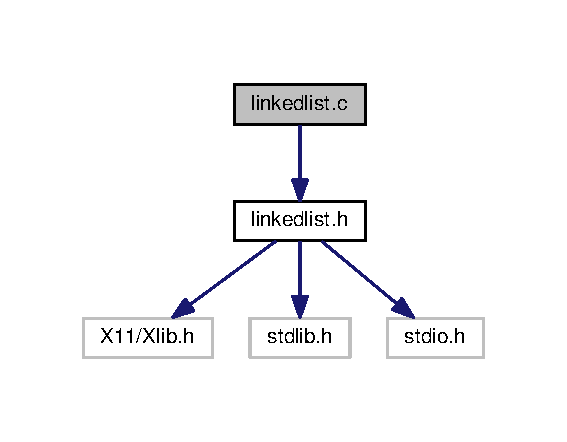
\includegraphics[width=272pt]{linkedlist_8c__incl}
\end{center}
\end{figure}
\subsection*{Functions}
\begin{DoxyCompactItemize}
\item 
void \hyperlink{linkedlist_8c_a46eaa6eca85d2d9a4c018a06ccaaeaf4}{insert} (\hyperlink{structNode}{Node} $\ast$new)
\item 
void \hyperlink{linkedlist_8c_a2feada6f7240f6f4e85116fb1301c0a9}{delete} (Window win\+I\+D)
\item 
int \hyperlink{linkedlist_8c_af61710f5d0837eacc50c2ecf8548cacd}{is\+In\+List} (Window win\+I\+D)
\item 
\hyperlink{structNode}{Node} $\ast$ \hyperlink{linkedlist_8c_a43cec99c147b276613e6e79abceeb4a7}{get\+Node\+From\+I\+D} (Window win\+I\+D)
\item 
void \hyperlink{linkedlist_8c_a1e5b20fed15743656bb6d2e6a6ea6269}{display} ()
\end{DoxyCompactItemize}
\subsection*{Variables}
\begin{DoxyCompactItemize}
\item 
\hyperlink{structNode}{Node} $\ast$ \hyperlink{linkedlist_8c_a2addc5f5fab651284199528b83cd61c8}{first}
\item 
\hyperlink{structNode}{Node} $\ast$ \hyperlink{linkedlist_8c_a16ac028724e4fd7016faa38928658477}{last}
\item 
int \hyperlink{linkedlist_8c_a892b640a9383f2428cade971e1164819}{window\+Count}
\end{DoxyCompactItemize}


\subsection{Function Documentation}
\hypertarget{linkedlist_8c_a2feada6f7240f6f4e85116fb1301c0a9}{}\index{linkedlist.\+c@{linkedlist.\+c}!delete@{delete}}
\index{delete@{delete}!linkedlist.\+c@{linkedlist.\+c}}
\subsubsection[{delete}]{\setlength{\rightskip}{0pt plus 5cm}void delete (
\begin{DoxyParamCaption}
\item[{Window}]{win\+I\+D}
\end{DoxyParamCaption}
)}\label{linkedlist_8c_a2feada6f7240f6f4e85116fb1301c0a9}
Delete a \hyperlink{structNode}{Node} from the list in the event that a window is detroyed given it\textquotesingle{}s I\+D. Update the total count of mapped windows. \hypertarget{linkedlist_8c_a1e5b20fed15743656bb6d2e6a6ea6269}{}\index{linkedlist.\+c@{linkedlist.\+c}!display@{display}}
\index{display@{display}!linkedlist.\+c@{linkedlist.\+c}}
\subsubsection[{display}]{\setlength{\rightskip}{0pt plus 5cm}void display (
\begin{DoxyParamCaption}
{}
\end{DoxyParamCaption}
)}\label{linkedlist_8c_a1e5b20fed15743656bb6d2e6a6ea6269}
Display the list in text, for debugging purposes. \hypertarget{linkedlist_8c_a43cec99c147b276613e6e79abceeb4a7}{}\index{linkedlist.\+c@{linkedlist.\+c}!get\+Node\+From\+I\+D@{get\+Node\+From\+I\+D}}
\index{get\+Node\+From\+I\+D@{get\+Node\+From\+I\+D}!linkedlist.\+c@{linkedlist.\+c}}
\subsubsection[{get\+Node\+From\+I\+D}]{\setlength{\rightskip}{0pt plus 5cm}{\bf Node}$\ast$ get\+Node\+From\+I\+D (
\begin{DoxyParamCaption}
\item[{Window}]{win\+I\+D}
\end{DoxyParamCaption}
)}\label{linkedlist_8c_a43cec99c147b276613e6e79abceeb4a7}
Given the window\textquotesingle{}s win\+I\+D, return the \hyperlink{structNode}{Node} that holds it. If it is not found, return N\+U\+L\+L. \hypertarget{linkedlist_8c_a46eaa6eca85d2d9a4c018a06ccaaeaf4}{}\index{linkedlist.\+c@{linkedlist.\+c}!insert@{insert}}
\index{insert@{insert}!linkedlist.\+c@{linkedlist.\+c}}
\subsubsection[{insert}]{\setlength{\rightskip}{0pt plus 5cm}void insert (
\begin{DoxyParamCaption}
\item[{{\bf Node} $\ast$}]{new}
\end{DoxyParamCaption}
)}\label{linkedlist_8c_a46eaa6eca85d2d9a4c018a06ccaaeaf4}
Insert a new \hyperlink{structNode}{Node} into the list and update the total count of mapped windows. Note that a node is always inserted at the front of the list. \hypertarget{linkedlist_8c_af61710f5d0837eacc50c2ecf8548cacd}{}\index{linkedlist.\+c@{linkedlist.\+c}!is\+In\+List@{is\+In\+List}}
\index{is\+In\+List@{is\+In\+List}!linkedlist.\+c@{linkedlist.\+c}}
\subsubsection[{is\+In\+List}]{\setlength{\rightskip}{0pt plus 5cm}int is\+In\+List (
\begin{DoxyParamCaption}
\item[{Window}]{win\+I\+D}
\end{DoxyParamCaption}
)}\label{linkedlist_8c_af61710f5d0837eacc50c2ecf8548cacd}
Return 1 if the window with the given win\+I\+D is in the list, otherwise return 0. 

\subsection{Variable Documentation}
\hypertarget{linkedlist_8c_a2addc5f5fab651284199528b83cd61c8}{}\index{linkedlist.\+c@{linkedlist.\+c}!first@{first}}
\index{first@{first}!linkedlist.\+c@{linkedlist.\+c}}
\subsubsection[{first}]{\setlength{\rightskip}{0pt plus 5cm}{\bf Node}$\ast$ first}\label{linkedlist_8c_a2addc5f5fab651284199528b83cd61c8}
Implementations of functions for manipulating a doubly, circular linked list holding X\+Lib Window I\+Ds. \hypertarget{linkedlist_8c_a16ac028724e4fd7016faa38928658477}{}\index{linkedlist.\+c@{linkedlist.\+c}!last@{last}}
\index{last@{last}!linkedlist.\+c@{linkedlist.\+c}}
\subsubsection[{last}]{\setlength{\rightskip}{0pt plus 5cm}{\bf Node}$\ast$ last}\label{linkedlist_8c_a16ac028724e4fd7016faa38928658477}
\hypertarget{linkedlist_8c_a892b640a9383f2428cade971e1164819}{}\index{linkedlist.\+c@{linkedlist.\+c}!window\+Count@{window\+Count}}
\index{window\+Count@{window\+Count}!linkedlist.\+c@{linkedlist.\+c}}
\subsubsection[{window\+Count}]{\setlength{\rightskip}{0pt plus 5cm}int window\+Count}\label{linkedlist_8c_a892b640a9383f2428cade971e1164819}

\hypertarget{linkedlist_8h}{}\section{linkedlist.\+h File Reference}
\label{linkedlist_8h}\index{linkedlist.\+h@{linkedlist.\+h}}
{\ttfamily \#include $<$X11/\+Xlib.\+h$>$}\\*
{\ttfamily \#include $<$stdlib.\+h$>$}\\*
{\ttfamily \#include $<$stdio.\+h$>$}\\*
Include dependency graph for linkedlist.\+h\+:\nopagebreak
\begin{figure}[H]
\begin{center}
\leavevmode
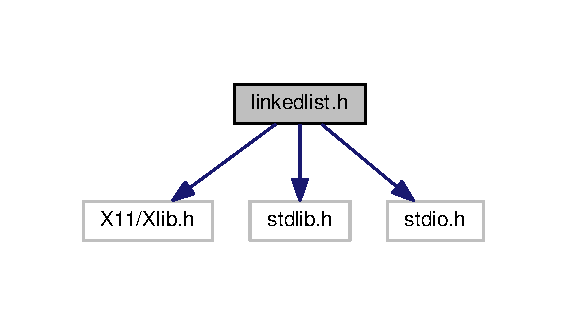
\includegraphics[width=272pt]{linkedlist_8h__incl}
\end{center}
\end{figure}
This graph shows which files directly or indirectly include this file\+:\nopagebreak
\begin{figure}[H]
\begin{center}
\leavevmode
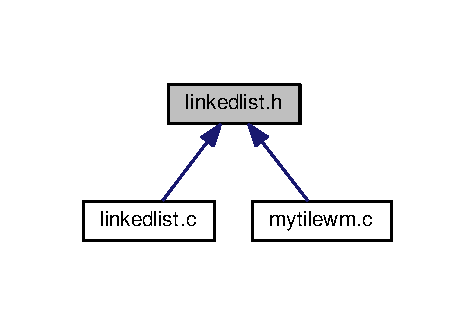
\includegraphics[width=228pt]{linkedlist_8h__dep__incl}
\end{center}
\end{figure}
\subsection*{Classes}
\begin{DoxyCompactItemize}
\item 
struct \hyperlink{structNode}{Node}
\end{DoxyCompactItemize}
\subsection*{Typedefs}
\begin{DoxyCompactItemize}
\item 
typedef struct \hyperlink{structNode}{Node} \hyperlink{linkedlist_8h_a3b09f37e675bcd48a01bf22155996872}{Node}
\end{DoxyCompactItemize}
\subsection*{Functions}
\begin{DoxyCompactItemize}
\item 
void \hyperlink{linkedlist_8h_a46eaa6eca85d2d9a4c018a06ccaaeaf4}{insert} (\hyperlink{structNode}{Node} $\ast$new)
\item 
void \hyperlink{linkedlist_8h_a2feada6f7240f6f4e85116fb1301c0a9}{delete} (Window win\+I\+D)
\item 
int \hyperlink{linkedlist_8h_af61710f5d0837eacc50c2ecf8548cacd}{is\+In\+List} (Window win\+I\+D)
\item 
\hyperlink{structNode}{Node} $\ast$ \hyperlink{linkedlist_8h_a43cec99c147b276613e6e79abceeb4a7}{get\+Node\+From\+I\+D} (Window win\+I\+D)
\item 
void \hyperlink{linkedlist_8h_a1e5b20fed15743656bb6d2e6a6ea6269}{display} ()
\end{DoxyCompactItemize}


\subsection{Typedef Documentation}
\hypertarget{linkedlist_8h_a3b09f37e675bcd48a01bf22155996872}{}\index{linkedlist.\+h@{linkedlist.\+h}!Node@{Node}}
\index{Node@{Node}!linkedlist.\+h@{linkedlist.\+h}}
\subsubsection[{Node}]{\setlength{\rightskip}{0pt plus 5cm}typedef struct {\bf Node} {\bf Node}}\label{linkedlist_8h_a3b09f37e675bcd48a01bf22155996872}


\subsection{Function Documentation}
\hypertarget{linkedlist_8h_a2feada6f7240f6f4e85116fb1301c0a9}{}\index{linkedlist.\+h@{linkedlist.\+h}!delete@{delete}}
\index{delete@{delete}!linkedlist.\+h@{linkedlist.\+h}}
\subsubsection[{delete}]{\setlength{\rightskip}{0pt plus 5cm}void delete (
\begin{DoxyParamCaption}
\item[{Window}]{win\+I\+D}
\end{DoxyParamCaption}
)}\label{linkedlist_8h_a2feada6f7240f6f4e85116fb1301c0a9}
Delete a \hyperlink{structNode}{Node} from the list in the event that a window is detroyed given it\textquotesingle{}s I\+D. Update the total count of mapped windows. \hypertarget{linkedlist_8h_a1e5b20fed15743656bb6d2e6a6ea6269}{}\index{linkedlist.\+h@{linkedlist.\+h}!display@{display}}
\index{display@{display}!linkedlist.\+h@{linkedlist.\+h}}
\subsubsection[{display}]{\setlength{\rightskip}{0pt plus 5cm}void display (
\begin{DoxyParamCaption}
{}
\end{DoxyParamCaption}
)}\label{linkedlist_8h_a1e5b20fed15743656bb6d2e6a6ea6269}
Display the list in text, for debugging purposes. \hypertarget{linkedlist_8h_a43cec99c147b276613e6e79abceeb4a7}{}\index{linkedlist.\+h@{linkedlist.\+h}!get\+Node\+From\+I\+D@{get\+Node\+From\+I\+D}}
\index{get\+Node\+From\+I\+D@{get\+Node\+From\+I\+D}!linkedlist.\+h@{linkedlist.\+h}}
\subsubsection[{get\+Node\+From\+I\+D}]{\setlength{\rightskip}{0pt plus 5cm}{\bf Node}$\ast$ get\+Node\+From\+I\+D (
\begin{DoxyParamCaption}
\item[{Window}]{win\+I\+D}
\end{DoxyParamCaption}
)}\label{linkedlist_8h_a43cec99c147b276613e6e79abceeb4a7}
Given the window\textquotesingle{}s win\+I\+D, return the \hyperlink{structNode}{Node} that holds it. If it is not found, return N\+U\+L\+L. \hypertarget{linkedlist_8h_a46eaa6eca85d2d9a4c018a06ccaaeaf4}{}\index{linkedlist.\+h@{linkedlist.\+h}!insert@{insert}}
\index{insert@{insert}!linkedlist.\+h@{linkedlist.\+h}}
\subsubsection[{insert}]{\setlength{\rightskip}{0pt plus 5cm}void insert (
\begin{DoxyParamCaption}
\item[{{\bf Node} $\ast$}]{new}
\end{DoxyParamCaption}
)}\label{linkedlist_8h_a46eaa6eca85d2d9a4c018a06ccaaeaf4}
Insert a new \hyperlink{structNode}{Node} into the list and update the total count of mapped windows. Note that a node is always inserted at the front of the list. \hypertarget{linkedlist_8h_af61710f5d0837eacc50c2ecf8548cacd}{}\index{linkedlist.\+h@{linkedlist.\+h}!is\+In\+List@{is\+In\+List}}
\index{is\+In\+List@{is\+In\+List}!linkedlist.\+h@{linkedlist.\+h}}
\subsubsection[{is\+In\+List}]{\setlength{\rightskip}{0pt plus 5cm}int is\+In\+List (
\begin{DoxyParamCaption}
\item[{Window}]{win\+I\+D}
\end{DoxyParamCaption}
)}\label{linkedlist_8h_af61710f5d0837eacc50c2ecf8548cacd}
Return 1 if the window with the given win\+I\+D is in the list, otherwise return 0. 
\hypertarget{mytilewm_8c}{}\section{mytilewm.\+c File Reference}
\label{mytilewm_8c}\index{mytilewm.\+c@{mytilewm.\+c}}
{\ttfamily \#include $<$stdio.\+h$>$}\\*
{\ttfamily \#include $<$stdlib.\+h$>$}\\*
{\ttfamily \#include $<$unistd.\+h$>$}\\*
{\ttfamily \#include $<$X11/\+Xlib.\+h$>$}\\*
{\ttfamily \#include $<$X11/\+Xutil.\+h$>$}\\*
{\ttfamily \#include $<$X11/\+Xos.\+h$>$}\\*
{\ttfamily \#include $<$X11/\+Xatom.\+h$>$}\\*
{\ttfamily \#include \char`\"{}config.\+h\char`\"{}}\\*
{\ttfamily \#include \char`\"{}linkedlist.\+h\char`\"{}}\\*
Include dependency graph for mytilewm.\+c\+:\nopagebreak
\begin{figure}[H]
\begin{center}
\leavevmode
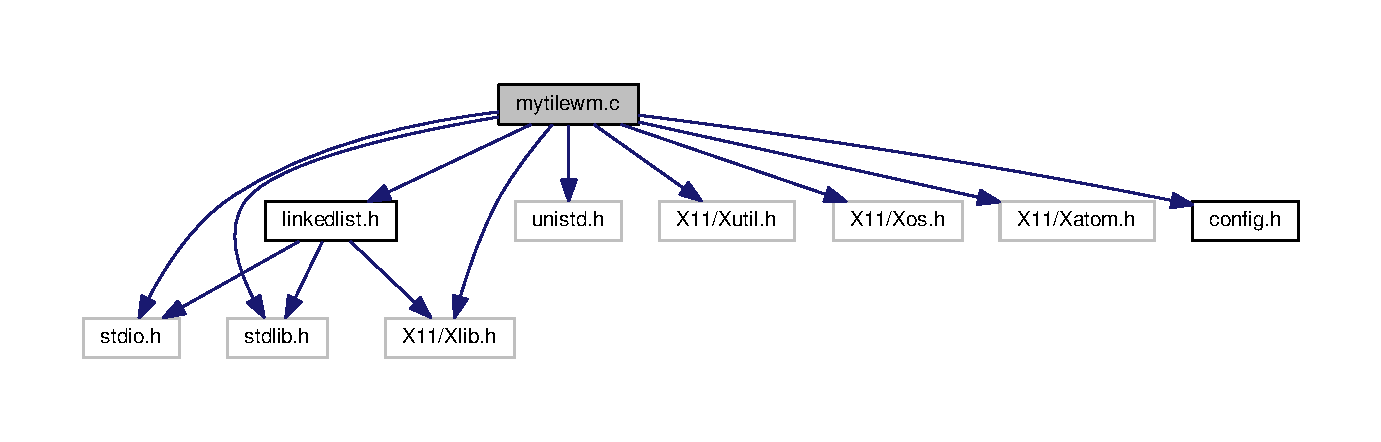
\includegraphics[width=350pt]{mytilewm_8c__incl}
\end{center}
\end{figure}
\subsection*{Classes}
\begin{DoxyCompactItemize}
\item 
struct \hyperlink{structWorkspace}{Workspace}
\end{DoxyCompactItemize}
\subsection*{Macros}
\begin{DoxyCompactItemize}
\item 
\#define \hyperlink{mytilewm_8c_afa99ec4acc4ecb2dc3c2d05da15d0e3f}{M\+A\+X}(a,  b)~((a) $>$ (b) ? (a) \+: (b))
\end{DoxyCompactItemize}
\subsection*{Enumerations}
\begin{DoxyCompactItemize}
\item 
enum \hyperlink{mytilewm_8c_a956154413ecb0b5bfa2bb8302116a1e8}{Tiling\+Algorithms} \{ \\*
\hyperlink{mytilewm_8c_a956154413ecb0b5bfa2bb8302116a1e8a3c25942291ac61d0c3611824f29cf928}{V\+S\+T\+A\+C\+K}, 
\hyperlink{mytilewm_8c_a956154413ecb0b5bfa2bb8302116a1e8a780bc5128a196fa7905fe6be80a428a3}{H\+S\+T\+A\+C\+K}, 
\hyperlink{mytilewm_8c_a956154413ecb0b5bfa2bb8302116a1e8ae0ef4285be2af9213b94b78159459698}{C\+O\+L\+S}, 
\hyperlink{mytilewm_8c_a956154413ecb0b5bfa2bb8302116a1e8a5f039f23ee85ddea038ca1ab88ca6755}{F\+U\+L\+L\+S\+C\+R\+E\+E\+N}, 
\\*
\hyperlink{mytilewm_8c_a956154413ecb0b5bfa2bb8302116a1e8ae064b4a6beaf71bfa759f063358ca104}{E\+X\+P\+E\+R\+I\+M\+E\+N\+T\+A\+L}
 \}
\end{DoxyCompactItemize}
\subsection*{Functions}
\begin{DoxyCompactItemize}
\item 
static void \hyperlink{mytilewm_8c_a5bb09e5de8bbbf8a29a08a77a560f295}{decrease\+Gaps} ()
\item 
static void \hyperlink{mytilewm_8c_ac95c2429dd3c26f2e268fa99e2c216f7}{increase\+Gaps} ()
\item 
static void \hyperlink{mytilewm_8c_ae3034c6b044829ed4e022f982728a5fa}{increase\+Main} ()
\item 
static void \hyperlink{mytilewm_8c_ae1187851b3af6c1ccf8e5396abb66a12}{decrease\+Main} ()
\item 
static void \hyperlink{mytilewm_8c_a258c78014043054d707f52202bc55929}{update\+Focus} ()
\item 
static void \hyperlink{mytilewm_8c_add501fd2303b12a79d769a71ae92adab}{focus\+Next} ()
\item 
static void \hyperlink{mytilewm_8c_ac132bc7aae05998ece3ec7cce99d3bd2}{focus\+Prev} ()
\item 
static void \hyperlink{mytilewm_8c_a0754204d6bad58bb8f7d3e05d938b6a8}{move\+Next} (\hyperlink{structNode}{Node} $\ast$current)
\item 
static void \hyperlink{mytilewm_8c_a82c52a525194d607a73acff738eb3fe4}{move\+Prev} (\hyperlink{structNode}{Node} $\ast$current)
\item 
static void \hyperlink{mytilewm_8c_a4862f865d956a758ae7f9d9d77660474}{float\+All\+Windows} ()
\item 
static int \hyperlink{mytilewm_8c_a6b49a9433aa79624109221549b0a5a25}{get\+Num\+Floating} ()
\item 
static void \hyperlink{mytilewm_8c_adf450a9a061d173710964aa7b86598b1}{tile} ()
\item 
static void \hyperlink{mytilewm_8c_ab1ae7940ad97d3a8f1102379e41d99b4}{force\+Tile} ()
\item 
static void \hyperlink{mytilewm_8c_a548635f166185d2fce65bf6a6d33bf5a}{experimental} ()
\item 
static void \hyperlink{mytilewm_8c_aaa22252f63245b6620b8a912d327261f}{vstack} ()
\item 
static void \hyperlink{mytilewm_8c_aa021adb516c76d35050d5595d08193ca}{hstack} ()
\item 
static void \hyperlink{mytilewm_8c_a3251f37cb11bd7dca82c6f8b225b0792}{columns} ()
\item 
static void \hyperlink{mytilewm_8c_a6a75e9b62aab932c6c357262257d370f}{grab\+Keys} ()
\item 
static void \hyperlink{mytilewm_8c_a01bd2b6f5f8a5acf7a702ece451b6f1b}{grab\+Buttons} ()
\item 
static void \hyperlink{mytilewm_8c_a597da1b6c0b49c7012fb605bbbf57434}{cycle\+Layouts} ()
\item 
static void \hyperlink{mytilewm_8c_a9e3b20d32b8ac810123bf75dc5247410}{send\+Destroy\+Message} ()
\item 
static void \hyperlink{mytilewm_8c_a39a4d6ec6164d2e5b961bbf1f922fd6c}{destroy\+Notify\+Event} ()
\item 
static void \hyperlink{mytilewm_8c_a5912ffa4b667b245b407b3b5e7a86a2a}{key\+Press\+Event} ()
\item 
static void \hyperlink{mytilewm_8c_a3f2fa4145cdd4e9fc79bb467ccb1e298}{button\+Press\+Event} ()
\item 
static void \hyperlink{mytilewm_8c_a1df6ccbcef300ae05e460104bb685f5b}{motion\+Notify\+Event} ()
\item 
static void \hyperlink{mytilewm_8c_aa283fbc81ec1beab2534b270f64f3526}{button\+Release\+Event} ()
\item 
static void \hyperlink{mytilewm_8c_a7634a382292bb511acf06c941bd66ed6}{map\+Request\+Event} ()
\item 
static void \hyperlink{mytilewm_8c_a57db02c4fba561c382037740b4eadd64}{configure\+Request\+Event} ()
\item 
static void \hyperlink{mytilewm_8c_a24b48bcda29b6ca2565c3cac5a09c13f}{swap\+Window\+Attributes} (Window x, Window y)
\item 
static unsigned long \hyperlink{mytilewm_8c_a8d5e042564d0c8ccad380cc11aa1485c}{get\+Pixel} ()
\item 
static int \hyperlink{mytilewm_8c_ab791e47d9d3d5fb48ad23b81b322da73}{get\+Key\+Code} (const char $\ast$key\+Name)
\item 
void \hyperlink{mytilewm_8c_a47dd1475ea792c2dacf0a4f3983bcc85}{fullscreen} ()
\item 
unsigned long \hyperlink{mytilewm_8c_a2970639e0c02e5990b3bd674d98a1785}{get\+Pixel} (const char $\ast$color\+Code)
\item 
int \hyperlink{mytilewm_8c_ae66f6b31b5ad750f1fe042a706a4e3d4}{main} ()
\end{DoxyCompactItemize}
\subsection*{Variables}
\begin{DoxyCompactItemize}
\item 
\hyperlink{structNode}{Node} $\ast$ \hyperlink{mytilewm_8c_a2addc5f5fab651284199528b83cd61c8}{first}
\item 
\hyperlink{structNode}{Node} $\ast$ \hyperlink{mytilewm_8c_a16ac028724e4fd7016faa38928658477}{last}
\item 
\hyperlink{structNode}{Node} $\ast$ \hyperlink{mytilewm_8c_a72b81f09bfa24192687a65d96f71705f}{curr\+Focus}
\item 
struct \hyperlink{structWorkspace}{Workspace} \hyperlink{mytilewm_8c_aeb497ff04fbbc6b79cece8980bf2ef36}{workspaces} \mbox{[}\hyperlink{config_8h_a7ed7c989849bb05c71d617e73cd05311}{N\+U\+M\+\_\+\+W\+O\+R\+K\+S\+P\+A\+C\+E\+S}\mbox{]}
\item 
Display $\ast$ \hyperlink{mytilewm_8c_a7d43b3edf58f8d85a89852ab95b740f6}{dpy}
\item 
int \hyperlink{mytilewm_8c_a3109b0889cec9f0de874a2bdc1f84372}{screen}
\item 
Window \hyperlink{mytilewm_8c_a67efd2aa4387dcb1b33df1f044512a16}{root}
\item 
int \hyperlink{mytilewm_8c_a892b640a9383f2428cade971e1164819}{window\+Count}
\item 
int \hyperlink{mytilewm_8c_ab9f00ec98f2f4c985581d76b371229e0}{G\+A\+P}
\item 
int \hyperlink{mytilewm_8c_ae615d5edd10587517b0daa1fe5179538}{P\+A\+N}
\item 
unsigned \hyperlink{mytilewm_8c_a5645d18f6655d7fe1c4e9295024d40a1}{screen\+Height}
\item 
unsigned \hyperlink{mytilewm_8c_a6a5a4b0e8a4d8d3c4c28d75f38365702}{screen\+Width}
\item 
X\+Event \hyperlink{mytilewm_8c_ad695247486d89834d82f80cea4f163dd}{event}
\item 
X\+Window\+Attributes \hyperlink{mytilewm_8c_a30c736fe26c351d7527f97c07646d70d}{attrs}
\item 
X\+Button\+Event \hyperlink{mytilewm_8c_a9420e02878dee7e6c5c82b04f33ecdc2}{start}
\item 
X\+Compose\+Status \hyperlink{mytilewm_8c_a7ab2edaf0279b16f5da849b9acb7fdcb}{compose}
\item 
char \hyperlink{mytilewm_8c_a5819dbc2d305e99e930c734a0d28bc3b}{buffer} \mbox{[}20\mbox{]}
\item 
int \hyperlink{mytilewm_8c_a52a25bb51473f2562b9d2b921d68ac52}{buffer\+Len} = 20
\item 
Key\+Sym \hyperlink{mytilewm_8c_a30c30b66c984b57e5f0c7e8148c49d43}{keysym}
\item 
char $\ast$ \hyperlink{mytilewm_8c_a28c6802e719f9b9ec42e06af122b1b48}{key\+A\+S\+C\+I\+I}
\item 
enum \hyperlink{mytilewm_8c_a956154413ecb0b5bfa2bb8302116a1e8}{Tiling\+Algorithms} \hyperlink{mytilewm_8c_a6687b37b92a0d3ec90d179844f7c4e84}{layout\+Mode}
\end{DoxyCompactItemize}


\subsection{Detailed Description}
\begin{DoxyAuthor}{Author}
Patrick Murphy 
\end{DoxyAuthor}


\subsection{Macro Definition Documentation}
\hypertarget{mytilewm_8c_afa99ec4acc4ecb2dc3c2d05da15d0e3f}{}\index{mytilewm.\+c@{mytilewm.\+c}!M\+A\+X@{M\+A\+X}}
\index{M\+A\+X@{M\+A\+X}!mytilewm.\+c@{mytilewm.\+c}}
\subsubsection[{M\+A\+X}]{\setlength{\rightskip}{0pt plus 5cm}\#define M\+A\+X(
\begin{DoxyParamCaption}
\item[{}]{a, }
\item[{}]{b}
\end{DoxyParamCaption}
)~((a) $>$ (b) ? (a) \+: (b))}\label{mytilewm_8c_afa99ec4acc4ecb2dc3c2d05da15d0e3f}


\subsection{Enumeration Type Documentation}
\hypertarget{mytilewm_8c_a956154413ecb0b5bfa2bb8302116a1e8}{}\index{mytilewm.\+c@{mytilewm.\+c}!Tiling\+Algorithms@{Tiling\+Algorithms}}
\index{Tiling\+Algorithms@{Tiling\+Algorithms}!mytilewm.\+c@{mytilewm.\+c}}
\subsubsection[{Tiling\+Algorithms}]{\setlength{\rightskip}{0pt plus 5cm}enum {\bf Tiling\+Algorithms}}\label{mytilewm_8c_a956154413ecb0b5bfa2bb8302116a1e8}
\begin{Desc}
\item[Enumerator]\par
\begin{description}
\index{V\+S\+T\+A\+C\+K@{V\+S\+T\+A\+C\+K}!mytilewm.\+c@{mytilewm.\+c}}\index{mytilewm.\+c@{mytilewm.\+c}!V\+S\+T\+A\+C\+K@{V\+S\+T\+A\+C\+K}}\item[{\em 
\hypertarget{mytilewm_8c_a956154413ecb0b5bfa2bb8302116a1e8a3c25942291ac61d0c3611824f29cf928}{}V\+S\+T\+A\+C\+K\label{mytilewm_8c_a956154413ecb0b5bfa2bb8302116a1e8a3c25942291ac61d0c3611824f29cf928}
}]\index{H\+S\+T\+A\+C\+K@{H\+S\+T\+A\+C\+K}!mytilewm.\+c@{mytilewm.\+c}}\index{mytilewm.\+c@{mytilewm.\+c}!H\+S\+T\+A\+C\+K@{H\+S\+T\+A\+C\+K}}\item[{\em 
\hypertarget{mytilewm_8c_a956154413ecb0b5bfa2bb8302116a1e8a780bc5128a196fa7905fe6be80a428a3}{}H\+S\+T\+A\+C\+K\label{mytilewm_8c_a956154413ecb0b5bfa2bb8302116a1e8a780bc5128a196fa7905fe6be80a428a3}
}]\index{C\+O\+L\+S@{C\+O\+L\+S}!mytilewm.\+c@{mytilewm.\+c}}\index{mytilewm.\+c@{mytilewm.\+c}!C\+O\+L\+S@{C\+O\+L\+S}}\item[{\em 
\hypertarget{mytilewm_8c_a956154413ecb0b5bfa2bb8302116a1e8ae0ef4285be2af9213b94b78159459698}{}C\+O\+L\+S\label{mytilewm_8c_a956154413ecb0b5bfa2bb8302116a1e8ae0ef4285be2af9213b94b78159459698}
}]\index{F\+U\+L\+L\+S\+C\+R\+E\+E\+N@{F\+U\+L\+L\+S\+C\+R\+E\+E\+N}!mytilewm.\+c@{mytilewm.\+c}}\index{mytilewm.\+c@{mytilewm.\+c}!F\+U\+L\+L\+S\+C\+R\+E\+E\+N@{F\+U\+L\+L\+S\+C\+R\+E\+E\+N}}\item[{\em 
\hypertarget{mytilewm_8c_a956154413ecb0b5bfa2bb8302116a1e8a5f039f23ee85ddea038ca1ab88ca6755}{}F\+U\+L\+L\+S\+C\+R\+E\+E\+N\label{mytilewm_8c_a956154413ecb0b5bfa2bb8302116a1e8a5f039f23ee85ddea038ca1ab88ca6755}
}]\index{E\+X\+P\+E\+R\+I\+M\+E\+N\+T\+A\+L@{E\+X\+P\+E\+R\+I\+M\+E\+N\+T\+A\+L}!mytilewm.\+c@{mytilewm.\+c}}\index{mytilewm.\+c@{mytilewm.\+c}!E\+X\+P\+E\+R\+I\+M\+E\+N\+T\+A\+L@{E\+X\+P\+E\+R\+I\+M\+E\+N\+T\+A\+L}}\item[{\em 
\hypertarget{mytilewm_8c_a956154413ecb0b5bfa2bb8302116a1e8ae064b4a6beaf71bfa759f063358ca104}{}E\+X\+P\+E\+R\+I\+M\+E\+N\+T\+A\+L\label{mytilewm_8c_a956154413ecb0b5bfa2bb8302116a1e8ae064b4a6beaf71bfa759f063358ca104}
}]\end{description}
\end{Desc}


\subsection{Function Documentation}
\hypertarget{mytilewm_8c_a3f2fa4145cdd4e9fc79bb467ccb1e298}{}\index{mytilewm.\+c@{mytilewm.\+c}!button\+Press\+Event@{button\+Press\+Event}}
\index{button\+Press\+Event@{button\+Press\+Event}!mytilewm.\+c@{mytilewm.\+c}}
\subsubsection[{button\+Press\+Event}]{\setlength{\rightskip}{0pt plus 5cm}void button\+Press\+Event (
\begin{DoxyParamCaption}
{}
\end{DoxyParamCaption}
)\hspace{0.3cm}{\ttfamily [static]}}\label{mytilewm_8c_a3f2fa4145cdd4e9fc79bb467ccb1e298}
For the handling of a \textquotesingle{}Button\+Press\textquotesingle{} X\+Event when it is received in the event loop. \hypertarget{mytilewm_8c_aa283fbc81ec1beab2534b270f64f3526}{}\index{mytilewm.\+c@{mytilewm.\+c}!button\+Release\+Event@{button\+Release\+Event}}
\index{button\+Release\+Event@{button\+Release\+Event}!mytilewm.\+c@{mytilewm.\+c}}
\subsubsection[{button\+Release\+Event}]{\setlength{\rightskip}{0pt plus 5cm}void button\+Release\+Event (
\begin{DoxyParamCaption}
{}
\end{DoxyParamCaption}
)\hspace{0.3cm}{\ttfamily [static]}}\label{mytilewm_8c_aa283fbc81ec1beab2534b270f64f3526}
For the handling of a \textquotesingle{}Button\+Release\textquotesingle{} X\+Event when it is received in the event loop. \hypertarget{mytilewm_8c_a3251f37cb11bd7dca82c6f8b225b0792}{}\index{mytilewm.\+c@{mytilewm.\+c}!columns@{columns}}
\index{columns@{columns}!mytilewm.\+c@{mytilewm.\+c}}
\subsubsection[{columns}]{\setlength{\rightskip}{0pt plus 5cm}void columns (
\begin{DoxyParamCaption}
{}
\end{DoxyParamCaption}
)\hspace{0.3cm}{\ttfamily [static]}}\label{mytilewm_8c_a3251f37cb11bd7dca82c6f8b225b0792}
Tile windows in such a way that all windows are equally sized, in a column fashion.

-- Fix issues in placement of windows \hypertarget{mytilewm_8c_a57db02c4fba561c382037740b4eadd64}{}\index{mytilewm.\+c@{mytilewm.\+c}!configure\+Request\+Event@{configure\+Request\+Event}}
\index{configure\+Request\+Event@{configure\+Request\+Event}!mytilewm.\+c@{mytilewm.\+c}}
\subsubsection[{configure\+Request\+Event}]{\setlength{\rightskip}{0pt plus 5cm}void configure\+Request\+Event (
\begin{DoxyParamCaption}
{}
\end{DoxyParamCaption}
)\hspace{0.3cm}{\ttfamily [static]}}\label{mytilewm_8c_a57db02c4fba561c382037740b4eadd64}
For the handling of a \textquotesingle{}Configure\+Request\textquotesingle{} X\+Event when it is received in the event loop. I was having issues with applications crashing after being mapped until I looked at some other window managers. Apparently, some programs must be configured with their desired configurations before it\textquotesingle{}s \textquotesingle{}safe\textquotesingle{} to impose our own. So, this function applies the application\textquotesingle{}s desired configuration and T\+H\+E\+N tiles (effectively undoing all that was set) to keep programs from crashing. \hypertarget{mytilewm_8c_a597da1b6c0b49c7012fb605bbbf57434}{}\index{mytilewm.\+c@{mytilewm.\+c}!cycle\+Layouts@{cycle\+Layouts}}
\index{cycle\+Layouts@{cycle\+Layouts}!mytilewm.\+c@{mytilewm.\+c}}
\subsubsection[{cycle\+Layouts}]{\setlength{\rightskip}{0pt plus 5cm}void cycle\+Layouts (
\begin{DoxyParamCaption}
{}
\end{DoxyParamCaption}
)\hspace{0.3cm}{\ttfamily [static]}}\label{mytilewm_8c_a597da1b6c0b49c7012fb605bbbf57434}
Cycle available tiling layouts. If there are windows to tile, \hyperlink{mytilewm_8c_adf450a9a061d173710964aa7b86598b1}{tile()} is called to apply the new layout. \hypertarget{mytilewm_8c_a5bb09e5de8bbbf8a29a08a77a560f295}{}\index{mytilewm.\+c@{mytilewm.\+c}!decrease\+Gaps@{decrease\+Gaps}}
\index{decrease\+Gaps@{decrease\+Gaps}!mytilewm.\+c@{mytilewm.\+c}}
\subsubsection[{decrease\+Gaps}]{\setlength{\rightskip}{0pt plus 5cm}void decrease\+Gaps (
\begin{DoxyParamCaption}
{}
\end{DoxyParamCaption}
)\hspace{0.3cm}{\ttfamily [static]}}\label{mytilewm_8c_a5bb09e5de8bbbf8a29a08a77a560f295}
Decrease the value of the G\+A\+P value (gaps between tiled windows) by G\+A\+P\+S\+\_\+\+I\+N\+C, and apply the change by retiling.

-- Add bounds checking \hypertarget{mytilewm_8c_ae1187851b3af6c1ccf8e5396abb66a12}{}\index{mytilewm.\+c@{mytilewm.\+c}!decrease\+Main@{decrease\+Main}}
\index{decrease\+Main@{decrease\+Main}!mytilewm.\+c@{mytilewm.\+c}}
\subsubsection[{decrease\+Main}]{\setlength{\rightskip}{0pt plus 5cm}void decrease\+Main (
\begin{DoxyParamCaption}
{}
\end{DoxyParamCaption}
)\hspace{0.3cm}{\ttfamily [static]}}\label{mytilewm_8c_ae1187851b3af6c1ccf8e5396abb66a12}
Decrease the size of the main window (horizontally) while tiled, then retile. \hypertarget{mytilewm_8c_a39a4d6ec6164d2e5b961bbf1f922fd6c}{}\index{mytilewm.\+c@{mytilewm.\+c}!destroy\+Notify\+Event@{destroy\+Notify\+Event}}
\index{destroy\+Notify\+Event@{destroy\+Notify\+Event}!mytilewm.\+c@{mytilewm.\+c}}
\subsubsection[{destroy\+Notify\+Event}]{\setlength{\rightskip}{0pt plus 5cm}void destroy\+Notify\+Event (
\begin{DoxyParamCaption}
{}
\end{DoxyParamCaption}
)\hspace{0.3cm}{\ttfamily [static]}}\label{mytilewm_8c_a39a4d6ec6164d2e5b961bbf1f922fd6c}
For the handling of a \textquotesingle{}Destroy\+Notify\textquotesingle{} X\+Event when it is received in the event loop. \hypertarget{mytilewm_8c_a548635f166185d2fce65bf6a6d33bf5a}{}\index{mytilewm.\+c@{mytilewm.\+c}!experimental@{experimental}}
\index{experimental@{experimental}!mytilewm.\+c@{mytilewm.\+c}}
\subsubsection[{experimental}]{\setlength{\rightskip}{0pt plus 5cm}void experimental (
\begin{DoxyParamCaption}
{}
\end{DoxyParamCaption}
)\hspace{0.3cm}{\ttfamily [static]}}\label{mytilewm_8c_a548635f166185d2fce65bf6a6d33bf5a}
\hypertarget{mytilewm_8c_a4862f865d956a758ae7f9d9d77660474}{}\index{mytilewm.\+c@{mytilewm.\+c}!float\+All\+Windows@{float\+All\+Windows}}
\index{float\+All\+Windows@{float\+All\+Windows}!mytilewm.\+c@{mytilewm.\+c}}
\subsubsection[{float\+All\+Windows}]{\setlength{\rightskip}{0pt plus 5cm}void float\+All\+Windows (
\begin{DoxyParamCaption}
{}
\end{DoxyParamCaption}
)\hspace{0.3cm}{\ttfamily [static]}}\label{mytilewm_8c_a4862f865d956a758ae7f9d9d77660474}
Float every window mapped to the screen.

-- Handle the issue of losing window focus indication after moving -- Handle issue of many windows causing offscreen stacking -- This command ought to be M\+O\+D + S\+H\+I\+F\+T + F \hypertarget{mytilewm_8c_add501fd2303b12a79d769a71ae92adab}{}\index{mytilewm.\+c@{mytilewm.\+c}!focus\+Next@{focus\+Next}}
\index{focus\+Next@{focus\+Next}!mytilewm.\+c@{mytilewm.\+c}}
\subsubsection[{focus\+Next}]{\setlength{\rightskip}{0pt plus 5cm}void focus\+Next (
\begin{DoxyParamCaption}
{}
\end{DoxyParamCaption}
)\hspace{0.3cm}{\ttfamily [static]}}\label{mytilewm_8c_add501fd2303b12a79d769a71ae92adab}
Change focus to the next window in the list (if windows exist). This involves setting the input focus with X\+Set\+Input\+Focus(), updating \textquotesingle{}curr\+Focus\textquotesingle{}, updating various window borders, and raising the newly focused window. \hypertarget{mytilewm_8c_ac132bc7aae05998ece3ec7cce99d3bd2}{}\index{mytilewm.\+c@{mytilewm.\+c}!focus\+Prev@{focus\+Prev}}
\index{focus\+Prev@{focus\+Prev}!mytilewm.\+c@{mytilewm.\+c}}
\subsubsection[{focus\+Prev}]{\setlength{\rightskip}{0pt plus 5cm}void focus\+Prev (
\begin{DoxyParamCaption}
{}
\end{DoxyParamCaption}
)\hspace{0.3cm}{\ttfamily [static]}}\label{mytilewm_8c_ac132bc7aae05998ece3ec7cce99d3bd2}
Change focus to the previous window in the list (if windows exist). This involves setting the input focus with X\+Set\+Input\+Focus(), updating \textquotesingle{}curr\+Focus\textquotesingle{}, updating various window borders, and raising the newly focused window. \hypertarget{mytilewm_8c_ab1ae7940ad97d3a8f1102379e41d99b4}{}\index{mytilewm.\+c@{mytilewm.\+c}!force\+Tile@{force\+Tile}}
\index{force\+Tile@{force\+Tile}!mytilewm.\+c@{mytilewm.\+c}}
\subsubsection[{force\+Tile}]{\setlength{\rightskip}{0pt plus 5cm}void force\+Tile (
\begin{DoxyParamCaption}
{}
\end{DoxyParamCaption}
)\hspace{0.3cm}{\ttfamily [static]}}\label{mytilewm_8c_ab1ae7940ad97d3a8f1102379e41d99b4}
Force a retile of all windows mapped to the screen. \hypertarget{mytilewm_8c_a47dd1475ea792c2dacf0a4f3983bcc85}{}\index{mytilewm.\+c@{mytilewm.\+c}!fullscreen@{fullscreen}}
\index{fullscreen@{fullscreen}!mytilewm.\+c@{mytilewm.\+c}}
\subsubsection[{fullscreen}]{\setlength{\rightskip}{0pt plus 5cm}void fullscreen (
\begin{DoxyParamCaption}
{}
\end{DoxyParamCaption}
)}\label{mytilewm_8c_a47dd1475ea792c2dacf0a4f3983bcc85}
Give the window full screen space (minus any gaps or borders)

-- minus the borders \hypertarget{mytilewm_8c_ab791e47d9d3d5fb48ad23b81b322da73}{}\index{mytilewm.\+c@{mytilewm.\+c}!get\+Key\+Code@{get\+Key\+Code}}
\index{get\+Key\+Code@{get\+Key\+Code}!mytilewm.\+c@{mytilewm.\+c}}
\subsubsection[{get\+Key\+Code}]{\setlength{\rightskip}{0pt plus 5cm}int get\+Key\+Code (
\begin{DoxyParamCaption}
\item[{const char $\ast$}]{key\+Name}
\end{DoxyParamCaption}
)\hspace{0.3cm}{\ttfamily [static]}}\label{mytilewm_8c_ab791e47d9d3d5fb48ad23b81b322da73}
Given the key name, convert to a Keysym, then convert to and return the Keycode. \hypertarget{mytilewm_8c_a6b49a9433aa79624109221549b0a5a25}{}\index{mytilewm.\+c@{mytilewm.\+c}!get\+Num\+Floating@{get\+Num\+Floating}}
\index{get\+Num\+Floating@{get\+Num\+Floating}!mytilewm.\+c@{mytilewm.\+c}}
\subsubsection[{get\+Num\+Floating}]{\setlength{\rightskip}{0pt plus 5cm}int get\+Num\+Floating (
\begin{DoxyParamCaption}
{}
\end{DoxyParamCaption}
)\hspace{0.3cm}{\ttfamily [static]}}\label{mytilewm_8c_a6b49a9433aa79624109221549b0a5a25}
Return the number of windows in the list currently marked as floating. \hypertarget{mytilewm_8c_a8d5e042564d0c8ccad380cc11aa1485c}{}\index{mytilewm.\+c@{mytilewm.\+c}!get\+Pixel@{get\+Pixel}}
\index{get\+Pixel@{get\+Pixel}!mytilewm.\+c@{mytilewm.\+c}}
\subsubsection[{get\+Pixel}]{\setlength{\rightskip}{0pt plus 5cm}static unsigned long get\+Pixel (
\begin{DoxyParamCaption}
{}
\end{DoxyParamCaption}
)\hspace{0.3cm}{\ttfamily [static]}}\label{mytilewm_8c_a8d5e042564d0c8ccad380cc11aa1485c}
\hypertarget{mytilewm_8c_a2970639e0c02e5990b3bd674d98a1785}{}\index{mytilewm.\+c@{mytilewm.\+c}!get\+Pixel@{get\+Pixel}}
\index{get\+Pixel@{get\+Pixel}!mytilewm.\+c@{mytilewm.\+c}}
\subsubsection[{get\+Pixel}]{\setlength{\rightskip}{0pt plus 5cm}unsigned long get\+Pixel (
\begin{DoxyParamCaption}
\item[{const char $\ast$}]{color\+Code}
\end{DoxyParamCaption}
)}\label{mytilewm_8c_a2970639e0c02e5990b3bd674d98a1785}
Return a pixel with the given color. \hypertarget{mytilewm_8c_a01bd2b6f5f8a5acf7a702ece451b6f1b}{}\index{mytilewm.\+c@{mytilewm.\+c}!grab\+Buttons@{grab\+Buttons}}
\index{grab\+Buttons@{grab\+Buttons}!mytilewm.\+c@{mytilewm.\+c}}
\subsubsection[{grab\+Buttons}]{\setlength{\rightskip}{0pt plus 5cm}void grab\+Buttons (
\begin{DoxyParamCaption}
{}
\end{DoxyParamCaption}
)\hspace{0.3cm}{\ttfamily [static]}}\label{mytilewm_8c_a01bd2b6f5f8a5acf7a702ece451b6f1b}
\textquotesingle{}Grab\textquotesingle{} the mouse buttons that the program will use. \hypertarget{mytilewm_8c_a6a75e9b62aab932c6c357262257d370f}{}\index{mytilewm.\+c@{mytilewm.\+c}!grab\+Keys@{grab\+Keys}}
\index{grab\+Keys@{grab\+Keys}!mytilewm.\+c@{mytilewm.\+c}}
\subsubsection[{grab\+Keys}]{\setlength{\rightskip}{0pt plus 5cm}void grab\+Keys (
\begin{DoxyParamCaption}
{}
\end{DoxyParamCaption}
)\hspace{0.3cm}{\ttfamily [static]}}\label{mytilewm_8c_a6a75e9b62aab932c6c357262257d370f}
\textquotesingle{}Grab\textquotesingle{} the keys that the program will use. \hypertarget{mytilewm_8c_aa021adb516c76d35050d5595d08193ca}{}\index{mytilewm.\+c@{mytilewm.\+c}!hstack@{hstack}}
\index{hstack@{hstack}!mytilewm.\+c@{mytilewm.\+c}}
\subsubsection[{hstack}]{\setlength{\rightskip}{0pt plus 5cm}void hstack (
\begin{DoxyParamCaption}
{}
\end{DoxyParamCaption}
)\hspace{0.3cm}{\ttfamily [static]}}\label{mytilewm_8c_aa021adb516c76d35050d5595d08193ca}
Tile windows in \textquotesingle{}horizontal stack\textquotesingle{} style (flipped version of vertical stack). \hypertarget{mytilewm_8c_ac95c2429dd3c26f2e268fa99e2c216f7}{}\index{mytilewm.\+c@{mytilewm.\+c}!increase\+Gaps@{increase\+Gaps}}
\index{increase\+Gaps@{increase\+Gaps}!mytilewm.\+c@{mytilewm.\+c}}
\subsubsection[{increase\+Gaps}]{\setlength{\rightskip}{0pt plus 5cm}void increase\+Gaps (
\begin{DoxyParamCaption}
{}
\end{DoxyParamCaption}
)\hspace{0.3cm}{\ttfamily [static]}}\label{mytilewm_8c_ac95c2429dd3c26f2e268fa99e2c216f7}
Increase the value of the G\+A\+P value (gaps between tiled windows) by G\+A\+P\+S\+\_\+\+I\+N\+C, and apply the change by retiling.

-- Add bounds checking \hypertarget{mytilewm_8c_ae3034c6b044829ed4e022f982728a5fa}{}\index{mytilewm.\+c@{mytilewm.\+c}!increase\+Main@{increase\+Main}}
\index{increase\+Main@{increase\+Main}!mytilewm.\+c@{mytilewm.\+c}}
\subsubsection[{increase\+Main}]{\setlength{\rightskip}{0pt plus 5cm}void increase\+Main (
\begin{DoxyParamCaption}
{}
\end{DoxyParamCaption}
)\hspace{0.3cm}{\ttfamily [static]}}\label{mytilewm_8c_ae3034c6b044829ed4e022f982728a5fa}
Increase the size of the main window (horizontally) while tiled, then retile. \hypertarget{mytilewm_8c_a5912ffa4b667b245b407b3b5e7a86a2a}{}\index{mytilewm.\+c@{mytilewm.\+c}!key\+Press\+Event@{key\+Press\+Event}}
\index{key\+Press\+Event@{key\+Press\+Event}!mytilewm.\+c@{mytilewm.\+c}}
\subsubsection[{key\+Press\+Event}]{\setlength{\rightskip}{0pt plus 5cm}void key\+Press\+Event (
\begin{DoxyParamCaption}
{}
\end{DoxyParamCaption}
)\hspace{0.3cm}{\ttfamily [static]}}\label{mytilewm_8c_a5912ffa4b667b245b407b3b5e7a86a2a}
For the handling of a \textquotesingle{}Keypress\textquotesingle{} event when it is received in the event loop. Catches the key combination pressed, and takes the appropriate action. \hypertarget{mytilewm_8c_ae66f6b31b5ad750f1fe042a706a4e3d4}{}\index{mytilewm.\+c@{mytilewm.\+c}!main@{main}}
\index{main@{main}!mytilewm.\+c@{mytilewm.\+c}}
\subsubsection[{main}]{\setlength{\rightskip}{0pt plus 5cm}int main (
\begin{DoxyParamCaption}
{}
\end{DoxyParamCaption}
)}\label{mytilewm_8c_ae66f6b31b5ad750f1fe042a706a4e3d4}
The main function initializes a display, grabs keys and buttons, selects which X\+Events to listen for, and runs the event loop. \hypertarget{mytilewm_8c_a7634a382292bb511acf06c941bd66ed6}{}\index{mytilewm.\+c@{mytilewm.\+c}!map\+Request\+Event@{map\+Request\+Event}}
\index{map\+Request\+Event@{map\+Request\+Event}!mytilewm.\+c@{mytilewm.\+c}}
\subsubsection[{map\+Request\+Event}]{\setlength{\rightskip}{0pt plus 5cm}void map\+Request\+Event (
\begin{DoxyParamCaption}
{}
\end{DoxyParamCaption}
)\hspace{0.3cm}{\ttfamily [static]}}\label{mytilewm_8c_a7634a382292bb511acf06c941bd66ed6}
For the handling of a \textquotesingle{}Map\+Request\textquotesingle{} X\+Event when it is received in the event loop. \hypertarget{mytilewm_8c_a1df6ccbcef300ae05e460104bb685f5b}{}\index{mytilewm.\+c@{mytilewm.\+c}!motion\+Notify\+Event@{motion\+Notify\+Event}}
\index{motion\+Notify\+Event@{motion\+Notify\+Event}!mytilewm.\+c@{mytilewm.\+c}}
\subsubsection[{motion\+Notify\+Event}]{\setlength{\rightskip}{0pt plus 5cm}void motion\+Notify\+Event (
\begin{DoxyParamCaption}
{}
\end{DoxyParamCaption}
)\hspace{0.3cm}{\ttfamily [static]}}\label{mytilewm_8c_a1df6ccbcef300ae05e460104bb685f5b}
For the handling of a \textquotesingle{}Motion\+Notify\textquotesingle{} X\+Event when it is received in the event loop. \hypertarget{mytilewm_8c_a0754204d6bad58bb8f7d3e05d938b6a8}{}\index{mytilewm.\+c@{mytilewm.\+c}!move\+Next@{move\+Next}}
\index{move\+Next@{move\+Next}!mytilewm.\+c@{mytilewm.\+c}}
\subsubsection[{move\+Next}]{\setlength{\rightskip}{0pt plus 5cm}void move\+Next (
\begin{DoxyParamCaption}
\item[{{\bf Node} $\ast$}]{current}
\end{DoxyParamCaption}
)\hspace{0.3cm}{\ttfamily [static]}}\label{mytilewm_8c_a0754204d6bad58bb8f7d3e05d938b6a8}
Move the window one position forward in the list. Note that the Nodes in in the list are not actually swapped, only a \hyperlink{structNode}{Node}\textquotesingle{}s win\+I\+D. \hypertarget{mytilewm_8c_a82c52a525194d607a73acff738eb3fe4}{}\index{mytilewm.\+c@{mytilewm.\+c}!move\+Prev@{move\+Prev}}
\index{move\+Prev@{move\+Prev}!mytilewm.\+c@{mytilewm.\+c}}
\subsubsection[{move\+Prev}]{\setlength{\rightskip}{0pt plus 5cm}void move\+Prev (
\begin{DoxyParamCaption}
\item[{{\bf Node} $\ast$}]{current}
\end{DoxyParamCaption}
)\hspace{0.3cm}{\ttfamily [static]}}\label{mytilewm_8c_a82c52a525194d607a73acff738eb3fe4}
Move the window one position backward in the list. Note that the Nodes in in the list are not actually swapped, only a \hyperlink{structNode}{Node}\textquotesingle{}s win\+I\+D. \hypertarget{mytilewm_8c_a9e3b20d32b8ac810123bf75dc5247410}{}\index{mytilewm.\+c@{mytilewm.\+c}!send\+Destroy\+Message@{send\+Destroy\+Message}}
\index{send\+Destroy\+Message@{send\+Destroy\+Message}!mytilewm.\+c@{mytilewm.\+c}}
\subsubsection[{send\+Destroy\+Message}]{\setlength{\rightskip}{0pt plus 5cm}void send\+Destroy\+Message (
\begin{DoxyParamCaption}
{}
\end{DoxyParamCaption}
)\hspace{0.3cm}{\ttfamily [static]}}\label{mytilewm_8c_a9e3b20d32b8ac810123bf75dc5247410}
Send a message to a client in hopes that it will close itself properly rather than simply killing the process. \hypertarget{mytilewm_8c_a24b48bcda29b6ca2565c3cac5a09c13f}{}\index{mytilewm.\+c@{mytilewm.\+c}!swap\+Window\+Attributes@{swap\+Window\+Attributes}}
\index{swap\+Window\+Attributes@{swap\+Window\+Attributes}!mytilewm.\+c@{mytilewm.\+c}}
\subsubsection[{swap\+Window\+Attributes}]{\setlength{\rightskip}{0pt plus 5cm}void swap\+Window\+Attributes (
\begin{DoxyParamCaption}
\item[{Window}]{x, }
\item[{Window}]{y}
\end{DoxyParamCaption}
)\hspace{0.3cm}{\ttfamily [static]}}\label{mytilewm_8c_a24b48bcda29b6ca2565c3cac5a09c13f}
Swaps window information, in other words, Window x will now have the coordinates and dimensions of Window y, and vice-\/versa. \hypertarget{mytilewm_8c_adf450a9a061d173710964aa7b86598b1}{}\index{mytilewm.\+c@{mytilewm.\+c}!tile@{tile}}
\index{tile@{tile}!mytilewm.\+c@{mytilewm.\+c}}
\subsubsection[{tile}]{\setlength{\rightskip}{0pt plus 5cm}void tile (
\begin{DoxyParamCaption}
{}
\end{DoxyParamCaption}
)\hspace{0.3cm}{\ttfamily [static]}}\label{mytilewm_8c_adf450a9a061d173710964aa7b86598b1}
Select the tiling layout based on \textquotesingle{}layout\+Mode\textquotesingle{} and tile the windows accordingly. \hypertarget{mytilewm_8c_a258c78014043054d707f52202bc55929}{}\index{mytilewm.\+c@{mytilewm.\+c}!update\+Focus@{update\+Focus}}
\index{update\+Focus@{update\+Focus}!mytilewm.\+c@{mytilewm.\+c}}
\subsubsection[{update\+Focus}]{\setlength{\rightskip}{0pt plus 5cm}void update\+Focus (
\begin{DoxyParamCaption}
{}
\end{DoxyParamCaption}
)\hspace{0.3cm}{\ttfamily [static]}}\label{mytilewm_8c_a258c78014043054d707f52202bc55929}
When the list of windows is altered -- by a deletion, for example -- the focus Must be updated. This involves setting the input focus with X\+Set\+Input\+Focus(), updating \textquotesingle{}curr\+Focus\textquotesingle{}, updating various window borders to indicate focus, and raising the newly focused window. \hypertarget{mytilewm_8c_aaa22252f63245b6620b8a912d327261f}{}\index{mytilewm.\+c@{mytilewm.\+c}!vstack@{vstack}}
\index{vstack@{vstack}!mytilewm.\+c@{mytilewm.\+c}}
\subsubsection[{vstack}]{\setlength{\rightskip}{0pt plus 5cm}void vstack (
\begin{DoxyParamCaption}
{}
\end{DoxyParamCaption}
)\hspace{0.3cm}{\ttfamily [static]}}\label{mytilewm_8c_aaa22252f63245b6620b8a912d327261f}
Tile windows in the classic \textquotesingle{}vertical stack\textquotesingle{} layout.

-- Try to redesign algorithm so tiling is done in single for loop. 

\subsection{Variable Documentation}
\hypertarget{mytilewm_8c_a30c736fe26c351d7527f97c07646d70d}{}\index{mytilewm.\+c@{mytilewm.\+c}!attrs@{attrs}}
\index{attrs@{attrs}!mytilewm.\+c@{mytilewm.\+c}}
\subsubsection[{attrs}]{\setlength{\rightskip}{0pt plus 5cm}X\+Window\+Attributes attrs}\label{mytilewm_8c_a30c736fe26c351d7527f97c07646d70d}
\hypertarget{mytilewm_8c_a5819dbc2d305e99e930c734a0d28bc3b}{}\index{mytilewm.\+c@{mytilewm.\+c}!buffer@{buffer}}
\index{buffer@{buffer}!mytilewm.\+c@{mytilewm.\+c}}
\subsubsection[{buffer}]{\setlength{\rightskip}{0pt plus 5cm}char buffer\mbox{[}20\mbox{]}}\label{mytilewm_8c_a5819dbc2d305e99e930c734a0d28bc3b}
\hypertarget{mytilewm_8c_a52a25bb51473f2562b9d2b921d68ac52}{}\index{mytilewm.\+c@{mytilewm.\+c}!buffer\+Len@{buffer\+Len}}
\index{buffer\+Len@{buffer\+Len}!mytilewm.\+c@{mytilewm.\+c}}
\subsubsection[{buffer\+Len}]{\setlength{\rightskip}{0pt plus 5cm}int buffer\+Len = 20}\label{mytilewm_8c_a52a25bb51473f2562b9d2b921d68ac52}
\hypertarget{mytilewm_8c_a7ab2edaf0279b16f5da849b9acb7fdcb}{}\index{mytilewm.\+c@{mytilewm.\+c}!compose@{compose}}
\index{compose@{compose}!mytilewm.\+c@{mytilewm.\+c}}
\subsubsection[{compose}]{\setlength{\rightskip}{0pt plus 5cm}X\+Compose\+Status compose}\label{mytilewm_8c_a7ab2edaf0279b16f5da849b9acb7fdcb}
\hypertarget{mytilewm_8c_a72b81f09bfa24192687a65d96f71705f}{}\index{mytilewm.\+c@{mytilewm.\+c}!curr\+Focus@{curr\+Focus}}
\index{curr\+Focus@{curr\+Focus}!mytilewm.\+c@{mytilewm.\+c}}
\subsubsection[{curr\+Focus}]{\setlength{\rightskip}{0pt plus 5cm}{\bf Node}$\ast$ curr\+Focus}\label{mytilewm_8c_a72b81f09bfa24192687a65d96f71705f}
\hypertarget{mytilewm_8c_a7d43b3edf58f8d85a89852ab95b740f6}{}\index{mytilewm.\+c@{mytilewm.\+c}!dpy@{dpy}}
\index{dpy@{dpy}!mytilewm.\+c@{mytilewm.\+c}}
\subsubsection[{dpy}]{\setlength{\rightskip}{0pt plus 5cm}Display$\ast$ dpy}\label{mytilewm_8c_a7d43b3edf58f8d85a89852ab95b740f6}
\hypertarget{mytilewm_8c_ad695247486d89834d82f80cea4f163dd}{}\index{mytilewm.\+c@{mytilewm.\+c}!event@{event}}
\index{event@{event}!mytilewm.\+c@{mytilewm.\+c}}
\subsubsection[{event}]{\setlength{\rightskip}{0pt plus 5cm}X\+Event event}\label{mytilewm_8c_ad695247486d89834d82f80cea4f163dd}
\hypertarget{mytilewm_8c_a2addc5f5fab651284199528b83cd61c8}{}\index{mytilewm.\+c@{mytilewm.\+c}!first@{first}}
\index{first@{first}!mytilewm.\+c@{mytilewm.\+c}}
\subsubsection[{first}]{\setlength{\rightskip}{0pt plus 5cm}{\bf Node}$\ast$ first}\label{mytilewm_8c_a2addc5f5fab651284199528b83cd61c8}
Implementations of functions for manipulating a doubly, circular linked list holding X\+Lib Window I\+Ds. \hypertarget{mytilewm_8c_ab9f00ec98f2f4c985581d76b371229e0}{}\index{mytilewm.\+c@{mytilewm.\+c}!G\+A\+P@{G\+A\+P}}
\index{G\+A\+P@{G\+A\+P}!mytilewm.\+c@{mytilewm.\+c}}
\subsubsection[{G\+A\+P}]{\setlength{\rightskip}{0pt plus 5cm}int G\+A\+P}\label{mytilewm_8c_ab9f00ec98f2f4c985581d76b371229e0}
\hypertarget{mytilewm_8c_a28c6802e719f9b9ec42e06af122b1b48}{}\index{mytilewm.\+c@{mytilewm.\+c}!key\+A\+S\+C\+I\+I@{key\+A\+S\+C\+I\+I}}
\index{key\+A\+S\+C\+I\+I@{key\+A\+S\+C\+I\+I}!mytilewm.\+c@{mytilewm.\+c}}
\subsubsection[{key\+A\+S\+C\+I\+I}]{\setlength{\rightskip}{0pt plus 5cm}char$\ast$ key\+A\+S\+C\+I\+I}\label{mytilewm_8c_a28c6802e719f9b9ec42e06af122b1b48}
\hypertarget{mytilewm_8c_a30c30b66c984b57e5f0c7e8148c49d43}{}\index{mytilewm.\+c@{mytilewm.\+c}!keysym@{keysym}}
\index{keysym@{keysym}!mytilewm.\+c@{mytilewm.\+c}}
\subsubsection[{keysym}]{\setlength{\rightskip}{0pt plus 5cm}Key\+Sym keysym}\label{mytilewm_8c_a30c30b66c984b57e5f0c7e8148c49d43}
\hypertarget{mytilewm_8c_a16ac028724e4fd7016faa38928658477}{}\index{mytilewm.\+c@{mytilewm.\+c}!last@{last}}
\index{last@{last}!mytilewm.\+c@{mytilewm.\+c}}
\subsubsection[{last}]{\setlength{\rightskip}{0pt plus 5cm}{\bf Node}$\ast$ last}\label{mytilewm_8c_a16ac028724e4fd7016faa38928658477}
\hypertarget{mytilewm_8c_a6687b37b92a0d3ec90d179844f7c4e84}{}\index{mytilewm.\+c@{mytilewm.\+c}!layout\+Mode@{layout\+Mode}}
\index{layout\+Mode@{layout\+Mode}!mytilewm.\+c@{mytilewm.\+c}}
\subsubsection[{layout\+Mode}]{\setlength{\rightskip}{0pt plus 5cm}enum {\bf Tiling\+Algorithms} layout\+Mode}\label{mytilewm_8c_a6687b37b92a0d3ec90d179844f7c4e84}
\hypertarget{mytilewm_8c_ae615d5edd10587517b0daa1fe5179538}{}\index{mytilewm.\+c@{mytilewm.\+c}!P\+A\+N@{P\+A\+N}}
\index{P\+A\+N@{P\+A\+N}!mytilewm.\+c@{mytilewm.\+c}}
\subsubsection[{P\+A\+N}]{\setlength{\rightskip}{0pt plus 5cm}int P\+A\+N}\label{mytilewm_8c_ae615d5edd10587517b0daa1fe5179538}
\hypertarget{mytilewm_8c_a67efd2aa4387dcb1b33df1f044512a16}{}\index{mytilewm.\+c@{mytilewm.\+c}!root@{root}}
\index{root@{root}!mytilewm.\+c@{mytilewm.\+c}}
\subsubsection[{root}]{\setlength{\rightskip}{0pt plus 5cm}Window root}\label{mytilewm_8c_a67efd2aa4387dcb1b33df1f044512a16}
\hypertarget{mytilewm_8c_a3109b0889cec9f0de874a2bdc1f84372}{}\index{mytilewm.\+c@{mytilewm.\+c}!screen@{screen}}
\index{screen@{screen}!mytilewm.\+c@{mytilewm.\+c}}
\subsubsection[{screen}]{\setlength{\rightskip}{0pt plus 5cm}int screen}\label{mytilewm_8c_a3109b0889cec9f0de874a2bdc1f84372}
\hypertarget{mytilewm_8c_a5645d18f6655d7fe1c4e9295024d40a1}{}\index{mytilewm.\+c@{mytilewm.\+c}!screen\+Height@{screen\+Height}}
\index{screen\+Height@{screen\+Height}!mytilewm.\+c@{mytilewm.\+c}}
\subsubsection[{screen\+Height}]{\setlength{\rightskip}{0pt plus 5cm}unsigned screen\+Height}\label{mytilewm_8c_a5645d18f6655d7fe1c4e9295024d40a1}
\hypertarget{mytilewm_8c_a6a5a4b0e8a4d8d3c4c28d75f38365702}{}\index{mytilewm.\+c@{mytilewm.\+c}!screen\+Width@{screen\+Width}}
\index{screen\+Width@{screen\+Width}!mytilewm.\+c@{mytilewm.\+c}}
\subsubsection[{screen\+Width}]{\setlength{\rightskip}{0pt plus 5cm}unsigned screen\+Width}\label{mytilewm_8c_a6a5a4b0e8a4d8d3c4c28d75f38365702}
\hypertarget{mytilewm_8c_a9420e02878dee7e6c5c82b04f33ecdc2}{}\index{mytilewm.\+c@{mytilewm.\+c}!start@{start}}
\index{start@{start}!mytilewm.\+c@{mytilewm.\+c}}
\subsubsection[{start}]{\setlength{\rightskip}{0pt plus 5cm}X\+Button\+Event start}\label{mytilewm_8c_a9420e02878dee7e6c5c82b04f33ecdc2}
\hypertarget{mytilewm_8c_a892b640a9383f2428cade971e1164819}{}\index{mytilewm.\+c@{mytilewm.\+c}!window\+Count@{window\+Count}}
\index{window\+Count@{window\+Count}!mytilewm.\+c@{mytilewm.\+c}}
\subsubsection[{window\+Count}]{\setlength{\rightskip}{0pt plus 5cm}int window\+Count}\label{mytilewm_8c_a892b640a9383f2428cade971e1164819}
\hypertarget{mytilewm_8c_aeb497ff04fbbc6b79cece8980bf2ef36}{}\index{mytilewm.\+c@{mytilewm.\+c}!workspaces@{workspaces}}
\index{workspaces@{workspaces}!mytilewm.\+c@{mytilewm.\+c}}
\subsubsection[{workspaces}]{\setlength{\rightskip}{0pt plus 5cm}struct {\bf Workspace} workspaces\mbox{[}{\bf N\+U\+M\+\_\+\+W\+O\+R\+K\+S\+P\+A\+C\+E\+S}\mbox{]}}\label{mytilewm_8c_aeb497ff04fbbc6b79cece8980bf2ef36}

\hypertarget{README_8md}{}\section{R\+E\+A\+D\+M\+E.\+md File Reference}
\label{README_8md}\index{R\+E\+A\+D\+M\+E.\+md@{R\+E\+A\+D\+M\+E.\+md}}

\hypertarget{utils_8h}{}\section{utils.\+h File Reference}
\label{utils_8h}\index{utils.\+h@{utils.\+h}}

%--- End generated contents ---

% Index
\backmatter
\newpage
\phantomsection
\clearemptydoublepage
\addcontentsline{toc}{chapter}{Index}
\printindex

\end{document}
